%%%%%%%%%%%%%%%%%%%%%%%%%%%%%%%%%%%%%%%%%%%%%%%%%%%%%%%%%%%%%%%%%%%%%%%%%%%%%%%%
%%                                                                            %%
%%                                                                            %%
%% Esimerkki opinnäytteen tekemisestä LaTeX:lla                               %%
%% Alkuperäinen versio ja nykinen kehitystyö Luis Costa, muutokset            %%
%% suomenkieliseen tekstipohjaan Perttu Puska.  							  %%
%% Tämän version on systeemianalyysin kanditöihin sopivaksi muokannut         %%
%% Juho Roponen. Uutena lisätty mm. fiplainnat.bst, joka                      %%
%% mahdollistaa suomenkielisten lähteiden kätevän käsittelyn    			  %%
%% .bib-tiedostolla.                                                          %%
%% Ruotsinkielen tuki lisätty 15092014                                        %%
%% PDF/A-1b -tuki lisätty 15092017                                            %%
%% PDF/A-2b -tuki lisätty 24042018                                            %%
%%                                                                            %%
%% Tähän esimerkkiin kuuluu tiedostot                                         %%
%%        opinnaytepohja.tex (versio 3.20) (opinnäytetyön pohja)              %%
%%        aaltothesis.cls (versio 3.20)                                       %%
%%        linediagram.eps                                                     %%
%%        curves.eps                                                          %%
%%        linediagram.pdf                                                     %%
%%        curves.pdf                                                          %%
%%        ledspole.jpg                                                        %%
%%                                                                            %%
%%                                                                            %%
%% Kääntäminen Linuxissa joko                                                 %%
%% pdflatex: (suositeltava tapa)                                              %%
%%             $ pdflatex opinnaytepohja                                      %%
%%             $ pdflatex opinnaytepohja                                      %%
%%                                                                            %%
%%   Tuloksena on tiedosto opinnaytepohja.pdf, joka on PDF/A-standardin       %%
%%   mukainen, jos olet valinnut oikeat \documentclass -optiot (kts. alla) ja %%
%%   ja käyttämäsi kuvatiedostoissa ei ole ongelmia.                          %%
%%                                                                            %%
%% Tai                                                                        %%
%% latex: (ei ole suositeltava tapa)                                          %%
%%             $ latex opinnaytepohja                                         %%
%%             $ latex opinnaytepohja                                         %%
%%                                                                            %%
%%   Tuloksena on tiedosto opinnayte.dvi, joka muutetaan ps-muotoon           %%
%%   seuraavasti                                                              %%
%%                                                                            %%
%%             $ dvips opinnaytepohja -o                                      %%
%%                                                                            %%
%%   ja edelleen pdf-muotoon seuraavasti                                      %%
%%                                                                            %%
%%             $ ps2pdf opinnaytepohja.ps                                     %%
%%                                                                            %%
%%   Tämä pdf EI ole pdf/a -tiedosto vaan se pitää muuttaa sellaiseksi esim.  %%
%%   Acrobat Pro- tai PDF-XChange -ohjelmalla.                                %%
%%                                                                            %%
%%                                                                            %%
%% Selittävät kommentit on tässä esimerkissä varustettu %%-merkeillä ja       %%
%% muutokset, joita käyttäjä voi tehdä, on varustettu %-merkeillä             %%
%%                                                                            %%
%%%%%%%%%%%%%%%%%%%%%%%%%%%%%%%%%%%%%%%%%%%%%%%%%%%%%%%%%%%%%%%%%%%%%%%%%%%%%%%%
%%%%%%%%%%%%%%%%%%%%%%%%%%%%%%%%%%%%%%%%%%%%%%%%%%%%%%%%%%%%%%%%%%%%%%%%%%%%%%%%
%%
%% MIKÄ on PDF/A?
%%
%% PDF/A on ISO-standardoitu versio pdf-tiedostosta. Standardin tavoite on, että
%% tiedosto on toistettavissa myös pitkänkin ajan kuluessa. PDF/A eroaa pdf:stä
%% siinä, että se sallii vain sellaisia pdf-ominaisuuksia, jotka tukevat
%% tiedoston pitkäaikaista arkistointia. Esim. PDF/A vaati, että kaikki käytetyt
%% fontit ovat mukana tiedostossa, mutta tavallisessa pdf:ssä voi olla niin,
%% että tiedostossa on vain linkki tiedostonlukijan tietokonejärjestelmän
%% fontteihin. PDF/A vaatii myös tietoa mm. värimäärittelystä ja käytetystä
%% salauksesta.
%% Tällä hetkellä PDF/A standardeja on kolme:
%% PDF/A-1: perustana PDF 1.4, standardi ISO19005-1, julkaistu vuonna 2005.
%%          Kaikki perusvaatimukset pitkäaikaiseen arkistointiin käytössä.
%% PDF/A-2: perustana PDF 1.7, standardi ISO19005-2, julkaistu vuonna 2011.
%%          Yllä olevan lisäksi tukee mm. OpenType-fonttien sisällyttämistä,
%%          läpinäkyvyyttä värimäärittelyssä ja digitaalisia allekirjoituksia.
%% PDF/A-3: perustana PDF 1.7, standardi ISO19005-3, julkaistu vuonna 2012.
%%          Eroaa edellisestä ainoastaan siinä, että se sallii missä tahansa
%%          tiedostoformaatissa (esim. xml, csv, cad, taulukkolaskentaformaatit,
%%          tekstinkäsittelyformaatit) olevien tiedostojen sisällyttämisen.
%% PDF/A-1 tiedostot eivät välttämättä ole PDF/A-2 -yhteensopivia eikä PDF/A-2
%% tiedostot ole PDF/A-1 -yhteensopivia.
%% Kaikista yllä olevista PDF/A-standardeista on kaksi tasoa:
%% b: (basic) vaatii, että tiedoston visuaalinen ilme on luotettavasti
%%    toistettavissa.
%% a: (accessible) b-tason vaatimuksien lisäksi, määrittelee kuinka saavutettava
%%    pdf-tiedosto on mm. vammaisteknologiaa hyödynttävissä ohjelmistoissa 
%%    (esim. kosketusruutua käytettävissä laitteissa).
%% Lisätietoa PDF/A:sta esim. https://en.wikipedia.org/wiki/PDF/A 
%%
%%
%% MINKÄ PDF/A -standardin mukaan teen opinnäytetyöni?
%%
%% Ensisijaisesti PDF/A-1b -standardin mukaan. Kuvaajat ja kuvat mitä
%% tyypillisesti käytetään opinnäytetyössä eivät tarvitse
%% läpinäkyvyysominaisuuksia. Perus '2D' -näkymä on riittävä. Opinnäytetyössä
%% käytettävät fontit on määritelty tässä pohjassa eikä niitä pidä muuttaa. Jos
%% käytät kuvia, jossa läpikäkyvyysominaisuuksillä on merkitystä, käytä PDF/A-2b
%% -standardia. Älä käytä PDF/A-3b -standardia opinnäytetyössäsi.
%%
%%
%% MITKÄ kuvaformaatteja voin käyttää PDF/A-tiedoston tekemisessä?
%%
%% Kun käytät pdflatexia työsi kääntämisessä suosi pdf-formaattia, mutta voit
%% käytä myös jpg- ja/tai png-formmaatia eteenkin valokuvissa.
%% Pdf-muotoisten kuvien kanssa voi tulla ongelmia PDF/A -yhteesopivuuden
%% kanssa, mm. jos fontit eivät ole upotettu tiedostoon.
%% Älä käytä PDF/A-formaattia kuvatiedostoissa.
%% Jos kuitenkin käytät perus latexia työsi kääntämisessä, ainoa sallittu
%% kuvaformaatti on eps. ÄLÄ käytä ps-formaattia kuvissasi.



%%%%%%%%%%%%%%%%%%%%%%%%%%%%%%%%%%%%%%%%%%
%%%%%% MUOKATTAVA OSUUS ALKAA TÄSTÄ %%%%%%
%%%%%%%%%%%%%%%%%%%%%%%%%%%%%%%%%%%%%%%%%%
%% KÄYTÄ näistä yhtä:
%% * ensimmäinen, jos käytät pdflatexia, joka kääntää tekstin suoraan
%%   pdf/a-tiedostoksi ja haluat julkaista opinnäytetyösi verkossa
%% * toinen, jos haluat tulostaa opinnäytteesi kansitettavaksi
%% * kolmas jos haluat tuottaa ps-tiedostoa ja siitä pdf/a:ta
%%
%% Kirjoita a.o. \documentclass optioiksi
%% * korkeakoulusi näistä: arts, biz, chem, elec, eng, sci
%% * editorisi käyttämä merkkikoodaustapa: utf8, latin1
%% * opinnäytetyön kieli: finnish, english, swedish
%% * tee arkistointikelpoinen PDF/A-1b tai PDF/A-2b pdf-tiedosto: a-1b, a-2b
%%                         (pdflatex tuottaa tavallisen metadataa sisältävän
%%                          pdf-tiedoston ilman a-*b optiota)
%% * verkkoon menevä symmetrinen taitto, sinisellä hypertekstillä: online  
%%                         (oletusarvo on leveä marginaali sivun sidonta
%%                          puolella ja musta hyperteksti)
%% * kaksipuolinen tulostus: twoside (oletusarvo on yksipuolinen tulostus)


\documentclass[finnish, 12pt, a4paper, sci, utf8, a-1b, online]{aaltothesis}
%\documentclass[finnish, 12pt, a4paper, sci, utf8, a-1b]{aaltothesis}

\usepackage{graphicx}
\usepackage{ifthen}

%% Matematiikan fontteja, symboleja ja muotoiluja lisää, näitä tarvitaan usein
\usepackage{amsfonts, amssymb, amsbsy, amsmath, mathrsfs, amsthm}
\usepackage{bbm}
\usepackage{changepage}

\theoremstyle{definition}
\newtheorem{definition}{Definition}[section] 
\newtheorem{aksiooma}[definition]{Aksiooma} 
\newtheorem{maaritelma}[definition]{Määritelmä}
\newtheorem{example}[definition]{Example}
\newtheorem{esimerkki}[definition]{Esimerkki}
\newtheorem{oivallus}{Oivallus}[section]
\newtheorem*{asetus}{Asetus}
\newtheorem*{ajatus}{Ajatus}
\newtheorem*{paatelma}{Päätelmä}

\theoremstyle{plain}
\newtheorem{theorem}[definition]{Theorem}
\newtheorem{lause}[definition]{Lause}
\newtheorem{lemma}[definition]{Lemma}
\newtheorem{apulause}[definition]{Apulause}
\newtheorem{corollary}[definition]{Corollary}
\newtheorem{seuraus}[definition]{Seurauslause}
\newtheorem{proposition}[definition]{Proposition}
\newtheorem{propositio}[definition]{Propositio}

\theoremstyle{remark}
\newtheorem{remark}[definition]{Remark}
\newtheorem{huomautus}[definition]{Huomautus}

\newcommand{\C}{\mathbb{C}}
\newcommand{\R}{\mathbb{R}}
\newcommand{\Q}{\mathbb{Q}}
\newcommand{\Z}{\mathbb{Z}}
\newcommand{\N}{\mathbb{N}}
\newcommand{\F}{\mathbb{F}}
\newcommand{\K}{\mathbb{K}}
\newcommand{\T}{\mathbb{T}}

\newcommand{\pallo}{\mathbb{S}}
\newcommand{\linkki}{\mathbf{L}}
\newcommand{\solmu}{\text{K}}
\newcommand{\interior}{\text{int }}
\newcommand{\syt}{\text{syt}}

\renewcommand{\P}{\mathbb{P}}
\renewcommand{\S}{\mathbb{S}}

%% Lähdeluettelon luomiseen
%% MainLang-muuttuja tulee aaltothesis.cls -tiedostosta ja sisältää 
%% sen kielen joka yllä on annettu documentclass-rivin parametrina
\usepackage[\MainLang]{babel}
\usepackage{natbib}
\usepackage{tikz}
\usetikzlibrary{cd}
\usetikzlibrary{babel}

\ifthenelse{\equal{\MainLang}{finnish}}{
\bibliographystyle{fiplainnat}
}{\ifthenelse{\equal{\MainLang}{english}}{
\bibliographystyle{plainnat}
}{\ifthenelse{\equal{\MainLang}{swedish}}{
\bibliographystyle{seplainnat}
}}{}}

\setcitestyle{authoryear,open={[},close={]}}
% use the below citestyle instead of the previous line if you want to use number citations as is common in mathematics: 
%\setcitestyle{numbers,open={[},close={]},comma}


%% Korjaa vastaamaan korkeakouluasi, jos automaattisesti asetettu nimi on
%% virheellinen. Annettu korkeakoulun nimi ei tule Aalto-logoon.
%%
%% Change the school field to specify your school if the automatically set name
%% is wrong. The specified school name will not be contained in the Aalto logo.
% \school{Korkeakouluni}

%% Korjaa seuraavat vastaamaan koulutusohjelmaasi
%%
\degreeprogram{Teknistieteellinen kandidaattiohjelma}
\major{Matematiikka ja systeemitieteet}
\code{SCI3029}
\univdegree{BSc}
\thesisauthor{Oscar Escartín}

%% Opinnäytteen otsikko tulee tähän.
%% Jos LaTeX ryhmittelee otsikon huonosti, voit joutua
%% pakottamaan rivinvaihdon \\ -kontrollimerkillä.
%% Tällöin...
%% - Muista että otsikkoja ei tavuteta! 
%% - Jos otsikossa on ja-sana, se ei jää rivin viimeiseksi sanaksi vaan aloittaa
%% uuden rivin.
%% - Anna ostikko uudelleen ilman rivinvaihtomerkkiä valinnaisena argumenttina
%% hakasuluissa. Näin tehdään, koska otsikko on osaa pdf/a-tiedostossa olevaa
%% metadataa, ja metadatassa ei saa olla rivinvaihtomerkkiä.
%%
\thesistitle{Opinnäytteen otsikko}
%\thesistitle[Opinnäytteen otsikko]{Opinnäyteen\\ otsikko}
%%

%%
\place{Espoo}
%%

%% Kandidaatintyön päivämäärä on sen esityspäivämäärä! 
%% 
\date{31.8.2018 {\color{red}KORJAA OIKEAKSI}}
%%

%% Kandidaatin- tai diplomityön valvoja.
%% Huomaa tittelissä "\" -merkki pisteen jälkeen, ennen välilyöntiä ja
%% seuraavaa merkkijonoa. 
%% Näin kerrotaan LaTeXille, että kyseessä ei ole lauseen loppu, jonka jälkeen
%% tulee hieman pidempi väli vaan halutaan tavallinen väli.
%%
\supervisor{Prof.\ Oscar Kivinen}
%%

%% Kandidaatintyön ohjaaja(t) tai diplomityön ohjaaja(t). Ohjaajia saa olla
%% korkeintaan kaksi. Todennäköisimmät tittelit suomeksi ja englanniksi:
%% Tekniikan tohtori: TkT / D.Sc. (Tech.) 
%% Diplomi-insinööri: DI / M.Sc. (Tech.)
\advisor{Prof.\ Oscar Kivinen}
%\advisor{DI Tina Tutkija}
%%


%% Tiivistelmä työn kielellä:
%% Kaikki tiivistelmässä tarvittava tieto (nimesi, työnnimi, jne.) käytetään
%% niin kuin se on yllä määritelty.
%%
%% Tiivistelmän avainsanat:
%% Huom! Avainsanat erotetaan tässä toisistaan \spc -makrolla jotta 
%% ne ovat metadatassa mukavassa muodossa
%% 
\keywords{Avainsanoiksi valitaan kirjoituksen\spc sisältöä keskeisesti\spc
	kuvaavia\spc käsitteitä}
%%

%% Tiivistelmän tekstiosa. Tämä teksti sisältyy pdf-tiedoston metadataan ja tulee
%% myös tiivistelmälomakkeeseen. Kirjoita tämä tiivistelmä työn kielellä.
%%
\thesisabstract{
Tiivistelmässä on lyhyt selvitys kirjoituksen tärkeimmästä sisällöstä: mitä ja
miten on tutkittu, sekä mitä tuloksia on saatu. Tämän opinnäytteen 
tiivistelmäteksti kirjoitetaan opinnäytteen luettavan osan
lomakkeen lisäksi myös pdf-tiedoston metadataan. Kirjoita tähän metadataan
kirjoitettava teksti. Metadatatekstissa ei saa olla erikoismerkkejä,
rivinvaihto- tai kappaleenjakomerkkiä, joten näitä merkkeja ei saa käyttää tässä.
Metadatatiivistelmätekstin on muuten oltava sama kuin lomakkeessa oleva teksti.
}
%%

%% Tekijänoikeusteksti. Tekijänoikeus on tekijällä riippumatta siitä onko
%% copyright -merkintä näkyvissä vai ei. Halutessasi voit jakaa työsi Creative
%% Commons -lisensillä (katso creativecommons.org), jolloin lisenssitekstin on
%% oltava näkyvissä. Kirjoita tähän haluamasi tekijänoikeustekti. Se kirjautuu
%% myös pdf-tiedoston metadataan.
%% Syntaksi:
%% \copyrigthtext{metadatateksti}{sivulle näkyviin tuleva teksti}
%%
%% A.o. metadataan menevässä tekstissä on käytettävä \noexpand -makroa ennen
%% \copyright -erikoismerkkiä ja lisäksi makrot (tässä \copyright ja \year) on
%% erotettava seuraavasta tekstistä \ -merkillä (välilyöntimerkki).
%% \copyrighttext-makron argumentissa olevat makrot automaattisesti hakevat
%% vuosiluvun ja tekijän nimi.
%% (Huom! \ThesisAuthor on aaltothesis.cls -tyylitiedoston sisäinen makro).
%% Toki saman tekstin olisi voinut kirjoittaa yksinkertaisesti näin:
%% \copyrighttext{Copyright \noexpand\copyright\ 2018 Teemu Teekkari}
%% {Copyright \copyright{} 2018 Teemu Teekkari}
%%
\copyrighttext{Copyright \noexpand\copyright\ \number\year\ \ThesisAuthor}
{Copyright \copyright{} \number\year{} \ThesisAuthor 
\\\\The document can be stored and made available to the public on the open internet pages of Aalto University.\\
All other rights are reserved.
}
%% Jos et halua työtäsin näkyviin systislabran verkkosivuille, poista 
%% copyright noticesta lupa jakaa työ Aallon verkkosivuilla.
%%

%% Voit estää LaTeXia kirjoittamasta xmpdata-tiedostoon (sisältää pdf
%% -tiedostoon kirjoitettavaa metadataa) asettamalla writexmpdatafile lipun
%% arvoksi 'false'. Tämä mahdollistaa sen, että voit kirjoittaa metadataa
%% suoraan oikeassa muodossa tiedostoon opinnaytepohja.xmpdata.
%%
%\setboolean{writexmpdatafile}{false}
%%


%% Kaikki mikä paperille tulostuu, on tämän jälkeen
\begin{document}
%% Tehdään kansilehti
%%

    \definecolor{aaltoBlack}{RGB}{0,0,0}%
    \definecolor{aaltoGray}{RGB}{140,133,123}%
    \definecolor{aaltoRed}{RGB}{239,51,64}%
    \definecolor{aaltoBlue}{RGB}{0,94,184}%
    \definecolor{aaltoYellow}{RGB}{255,205,0}%
    % Additional colors
    \definecolor{aaltoPurple}{RGB}{117,59,189}%
    \definecolor{aaltoGreen}{RGB}{0,150,94}%
    \definecolor{aaltoLightGreen}{RGB}{120,190,32}%
    \definecolor{aaltoOrange}{RGB}{255,103,31}%
    \definecolor{aaltoLightOrange}{RGB}{255,165,0}%
    \definecolor{aaltoFuchsia}{RGB}{187,22,163}%
\pagecolor{aaltoOrange} %Voit poistaa tämän, jollet halua värillistä kansilehteä
{%\color{white}
\uselogo{black}{''}

\makecoverpage{}
}
\nopagecolor
\uselogo{black}{''}

%% Tehdään tekijänoikeusteksti näkyväksi.
%% Halutessasi voit jättää tekijänoikeustekstin pois luettavasta pdf
%% -tiedostosta. Tämä voi tuntua hyvältä ajatukselta paperille tulostetulla
%% versiossa eteenkin, jos sivun ainoa teksti on "Copyright (c) vvvv Teemu 
%% Teekkari". Suositus on kuitenkin jättää teksti näkyviin.
%%
\makecopyrightpage{}

%% Tiivistelmä työn kielellä
%% Kaikki tiivistelmässä tarvittava tieto (nimesi, työnnimi, jne.) käytetään
%% niin kuin se on yllä määritelty.
%%
%% Tiivistelmän tekstiosa
\begin{abstractpage}
Tiivistelmässä on lyhyt selvitys kirjoituksen tärkeimmästä sisällöstä: mitä ja
miten on tutkittu, sekä mitä tuloksia on saatu.

Tämän opinnäytteen tiivistelmäteksti kirjoitetaan opinnäytteen luettavan osan 
lomakkeen lisäksi myös pdf-tiedoston metadataan 
$\backslash$thesisabstract-makron avulla (katso yllä). Kirjoita tähän
luettavaan tiivistelmälomakkeeseen menevä teksti. Tässä saa olla erikoismerkkejä
kuten kreikkalaiset kirjaimet ja rivinvaihto- ja kappaleenjakomerkit. Tämän
tekstin on muuten oltava sama kuin metedatatiivistelmän teksti.

Jos tiivistelmäsi ei sisällä erikoismerkkejä eikä kaipaa kappaleenjakoa, voit
hyödyntää makroa $\backslash$abstracttext joka käyttää ylläantamaasi 
metedata-kelpoista tiivistelmää (katso kommentti alla).

\end{abstractpage}

%% \thesisabstract -makrossa kirjoitettu teksti on tallennettu makroon
%% \abstracttext, jolloin voit siirtää metadataan menevän tekstin 
%% sellaisenaan näin:
%%
%\begin{abstractpage}
%	\abstracttext{}
%\end{abstractpage}




%% Pakotetaan uusi sivu varmuuden vuoksi, jotta tiivistelmät
%% eivät tule vahingossakaan samalle sivulle
\newpage
%% Opinnäytteen toinen tiivistelmä 
%% Mikäli opinnäytteen kieli on englanti, kirjoitetaan tämä 
%% tiivistelmä koulusivistyskielellä (suomi/ruotsi).
%% Mikäli taas opinnäyte on kirjoitettu koulusivistyskielellä,
%% suositellaan englanninkielisen tiivistelmän kirjoittamista.
%%
%% Päivitetään metatieto uudelle kielelle.
\thesistitle{Thesis template}
\supervisor{Prof.\ Oscar Kivinen}
\advisor{Prof.\ Oscar Kivinen}
%\advisor{MSc\ Tiina Tutkija}
\degreeprogram{Teknistieteellinen kandidaattiohjelma}
\major{Matematiikka ja systeemitieteet}
%% Avainsanoja ei tarvitse tässä erottaa \spc -makrolla.
\keywords{Resistor, resistance, temperature}
%% Tiivistelmän tekstiosa
\begin{abstractpage}[english] % finnish/swedish/english tarpeen mukaan
Your abstract in English. Keep the abstract short. The abstract explains your
research topic, the methods you have used, and the results you obtained.
\end{abstractpage}

%% Esipuhe 
%%
%% Tämä osio on vapaaehtoinen.
%%
%\mysection{Esipuhe}
%
%Haluan kiittää Professori Pirjo Professoria ja ohjaajaani Olli Ohjaajaa hyvästä
%ja huonosta ohjauksesta.\\
%
%\vspace{5cm}
%Otaniemi, 31.8.2018
%
%\vspace{5mm}
%{\hfill Teemu T.\ A.\ Teekkari \hspace{1cm}}

%% Pakotetaan varmuuden vuoksi esipuheen jälkeinen osa alkamaan uudelta sivulta
%\newpage


%% Sisällysluettelo
\thesistableofcontents


%% Symbolit ja lyhenteet
%\mysection{Symbolit ja lyhenteet}
%
%\subsection*{Symbolit}
%
%\begin{tabular}{ll}
%$\mathbf{B}$  & magneettivuon tiheys  \\
%$c$              & valon nopeus tyhjössä $\approx 3\times10^8$ [m/s]\\
%$\omega_{\mathrm{D}}$    & Debye-taajuus \\
%$\omega_{\mathrm{latt}}$ & hilan keskimääräinen fononitaajuus \\
%$\uparrow$       & elektronin spinin suunta ylöspäin\\
%$\downarrow$     & elektronin spinin suunta alaspäin
%\end{tabular}
%
%\subsection*{Operaattorit}
%
%\begin{tabular}{ll}
%$\nabla \times \mathbf{A}$              & vektorin $\mathbf{A}$ roottori\\
%$\displaystyle\frac{\mbox{d}}{\mbox{d} t}$ & derivaatta muuttujan $t$ 
%suhteen\\[3mm]
%$\displaystyle\frac{\partial}{\partial t}$  & osittaisderivaatta muuttujan $t$ 
%suhteen \\[3mm]
%$\sum_i $                       & summa indeksin $i$ yli\\
%$\mathbf{A} \cdot \mathbf{B}$    & vektorien $\mathbf{A}$ ja $\mathbf{B}$ 
%pistetulo
%\end{tabular}
%
%\subsection*{Lyhenteet}
%
%\begin{tabular}{ll}
%AC         & vaihtovirta \\
%APLAC      & an object-oriented analog circuit simulator and design tool \\
%           & (originally Analysis Program for Linear Active Circuits) \\
%BCS        & Bardeen-Cooper-Schrieffer \\ %% tavuviiva - nimien välissä 
%DC         & tasavirta \\
%TEM        & transverse eletromagnetic
%\end{tabular}


%% \clearpage on melkein samanlainen kuin \newpage, mutta flushaa myös LaTeX:n
%% floatit 
%% 
\cleardoublepage

%% Leipäteksti alkaa
%% \input-rivi korvautuu määritellyn tiedoston sisällöllä, tämä on helppo tapa
%% tehdä tiedostorakenteesta selkeämpi sen sijaan että koko leipäteksti olisi
%% päätiedostossa. Suositeltavaa on tehdä jokaiselle luvulle oma tiedosto ja 
%% nimetä ne järkevästi, alla esimerkki viidellä luvulla laitoksen 
%% kirjoitusohjeita mukaillen

\section{Johdanto}

Merkintätapoja.
\begin{itemize}
    \item $\approx$ homeomorfismi
    \item $\linkki,\solmu$ linkki ja solmu
    \item $N(\linkki),N(\solmu)$ linkin ja solmun putkiympäristö
    \item $M_i,L_i$ linkin osasen pituus- ja leveyspiiri
    \item $\#$ topologisten monistojen yhtenäinen summa
    \item 
\end{itemize}

Tämän tekstin lähteenä oleva tiedosto on opinnäytteen pohja, jota voi käyttää
kandidaatintyössä, diplomityössä ja lisensiaatintyössä. Tekstin lähteenä oleva
tiedosto on kirjoitettu \LaTeX-tiedoston rakenteen opiskelemista ajatellen.
Tiedoston kommentit sisältävät tietoa, joka on hyödyllistä opinnäytettä
kirjoitettaessa. 

%% Esimerkki luettelosta. Lyhyt ajatusviiva on käytössä luettelossa, ja se on
%% pituudeltaan en dash. Merkitään latex-koodissa --. 
Johdanto selvittää samat asiat kuin tiivistelmä, mutta laveammin. Johdannossa
kerrotaan yleensä seuraavat asiat

\begin{itemize}
\item[--]Tutkimuksen taustaa ja tutkimusaiheen yleisluonteinen esittely
\item[--]Tutkimuksen tavoitteet
\item[--]Pääkysymys ja osaongelmat
\item[--]Tutkimuksen rajaus ja keskeiset käsitteet.
\end{itemize}

Lyhyiden opinnäytteiden johdannot ovat yleensä liian pitkiä, joten johdannon
paisuttamista on vältettävä. Diplomityöhön sopii johdanto, joka on 2--4 sivua.
%% tässä on myös lyhyt ajatusviiva l. en dash.
Kandidaatintyön johdannon on oltava diplomityön johdantoa lyhyempi. Sopivasti
tiivistetty johdanto ei kaipaa alaotsikoita.

\begin{lause}
    \label{lause:päätulos}
    (i) Pelkistetty algebrallinen käyrä $V\subset\C^2$ jollakin upotuksella $\C^2\subset\P^2$ määrittää RPI-pujoskaavion $\Omega$ $V$:n äärettömyyslinkille. Äärettömyyspisteiden lukumäärälle pätee $n_\infty(V)=n$, missä $n$ on kaavion juurisilmun valenssi. Lisäksi $\deg(V)=\ell_\text{root}$, jossa $\ell_\text{root}$ on juuren (virtuaalisen) komponentin linkkiluku äärettömyyslinkin kanssa. Jos $V$ on säännöllinen käyrä, $\Omega$ on säännöllinen (määritelmä???) pujoskaavio.

    (ii) Linkki on jonkin äärettömyyslinkin (joka voidaan valita säännölliseksi (määritelmä???), jopa hyväksi (määritelmä???)) osalinkki jos ja vain jos sillä on RPI-pujoskaavio.
\end{lause}
\begin{ajatus}
    Lause on sangen tiukasti muotoiltu, mutta sen ydinajatus on seuraava.
    \begin{enumerate}[i]
        \item Minkälainen solmu tai pujoskaavio algebrallisella käyrällä on?
        \item Millä ehdoilla algebralliset käyrät vastaavat linkkejä ja pujoskaavioita yksi yhteen?
    \end{enumerate}
\end{ajatus}
\section{Differentiaaligeometriaa}
Käyrien muodostamien linkkien tutkimiseen tarvitaan (sileiden) monistojen teoriaa. Monistot ovat geometrisia rakenteita, jotka muistuttavat paikallisesti euklidista avaruutta. Ne mahdollistavat \emph{avaruuden rakenteen} käsitteen. Algebrallisten solmujen kannalta tämä on olennaista, sillä solmujen tutkimista helpottaa niiden upottaminen monistoon. Tässä työssä noudatetaan lähteen \citep{Lee2012} merkintätapoja.
\begin{huomautus}
    Tässä osiossa, kuten kirjallisuudessa yleisesti, käsitellään $\R$-monistoja, vaikka työ muuten käsittelee $\C$-käyriä. Monistojen teoria sellaisenaan ei kuitenkaan välitä skalaareiden reaalisuudesta, ja isomorfia $\C\cong\R^2$ sallii teorian siirtämisen kompleksiluvuille.
\end{huomautus}

\subsection{Sileät monistot ja Seifert-monisto}
Sileiden monistojen määrittely on jotakuinkin teknistä niiden ymmärrettävyyteen verrattuna. Kärsimätön lukija voi ohittaa osion, ja ajatella monistoja $n$-ulotteisina pintoina, jotka $n+1$-ulotteiseen avaruuteen upotettuna näyttävät paikallisesti $n$-ulotteisilta tasoilta, mutta saattavat globaalisti olla vääntyneitä.

Sileä monisto on sellainen monisto, joka ei ole ``rutussa'', jolloin sen pinnalla voi integroida ja derivoida käyriä. Esimerkiksi maapallo on sileä 2-ulotteinen monisto.
\begin{maaritelma}
    Olkoon $M$ topologinen avaruus. $M$ on \emph{$n$-ulotteinen topologinen monisto}, jos
    \begin{itemize}
        \item $M$ on Hausdorff-avaruus
        \item $M$ on $N_2$-avaruus
        \item $M$ on paikallisesti euklidisesti $n$-ulotteinen: kaikilla $p\in M$ on avoin ympäristö $U\subset M$, joka on homeomorfinen johonkin $\R^n$:n avoimeen osajoukkoon $V\subset\R^n$.
    \end{itemize}
\end{maaritelma}
\begin{huomautus}
    Yleisesti kirjoitetaan ``olkoon $M^n$ monisto'', jolla tarkoitetaan, että $M$ on $n$-ulotteinen monisto.
\end{huomautus}
\begin{esimerkki}
    Esimerkiksi Maapallo on 2-ulotteinen monisto, koska paikallisesti Maapallon pinta muistuttaa tasoa. Maapallo on erityistapaus algebrallisesta pinnasta, koska sen polynomiyhtälö $x^2+y^2+z^2=R^2$.
\end{esimerkki}
\begin{maaritelma}
    Olkoon $M^n$ monisto. $M$:n \emph{koordinaattikartta} on pari $(U,\varphi)$, jossa $U\subset M$ on avoin ja $\varphi:U\to\hat U$ on homeomorfismi avoimeen joukkoon $\hat U\subset R^n$. Koordinaattikartan \emph{koordinaattikuvaus} on $\varphi$.
\end{maaritelma}
\begin{esimerkki}
    Yleisesti algebrallinen hyperpinta $f(x_1,x_2,\dots,x_{n+1})=0$ määrittää $n$-ulotteisen moniston $\R^{n+1}$:ssä.
\end{esimerkki}
\begin{maaritelma}
    Jos $U\subset\R^n,V\subset\R^m$, funktio $f:U\to V$ on \emph{sileä}, jos sen jokaisella komponenttifunktiolla on jatkuvat asteen $n$ osittaisderivaatat kaikilla $n\in\N$.
\end{maaritelma}
\begin{maaritelma}
    Kuvaus $f:A\to B$ on \emph{diffeomorfismi}, jos $f$ on bijektio ja $f$ ja $f^{-1}$ ovat sileitä.
\end{maaritelma}
\begin{maaritelma}
    Moniston $M$ \emph{atlas} $\mathcal{A}$ on kokoelma karttoja $\{(U_i,\varphi_i)\}_{i\in I}$ siten, että karttojen lähtöjoukot peittävät moniston $M$: kaikille $p\in M$ on olemassa $i\in I$, jolle $p\in U_i$. Jos koordinaattikartat ovat pareittain sileästi yhteensopivia, eli
    \begin{equation}
        \varphi_j\circ\varphi_i^{-1}:\varphi_i(U_i\cap U_j)\to\varphi_j(U_i\cap U_j)
    \end{equation}
    tai $U_i\cap U_j=\emptyset$, niin $\mathcal{A}$ on \emph{sileä atlas}.
\end{maaritelma}
\begin{maaritelma}
    Monisto $M$ on \emph{sileä monisto}, jos sillä on sileä atlas.
\end{maaritelma}
Osion loppuhuipennuksena määritellään Seifert-monisto. 3-monistojen modernia teoriaa tuntemattomalle lukijalle määritelmä on käsittämätön, mutta käytännössä määritelmällä eritellään tutkimuksen kohteeksi mahdollisimman laaja monistojen joukko, joka käyttäytyisi mahdollisimman hyvin.
\begin{maaritelma}[Seifert-monisto ja Seifert-kuidutettu avaruus]
    \emph{Seifert-monisto} on 3-monisto, jonka voi pujontaoperaatiolla (määritelmä~\ref{maar:pujos}) rakentaa \emph{Seifert-kuidutetuista avaruuksista}, ts. avaruuksista, jotka voidaan esittää erillisten ympyröiden $\S^1$ yhdisteenä.
\end{maaritelma}
\begin{esimerkki}
    Sekä ontto että täytetty torus $\S^1\times\S^1$, $\S^1\times D^2$ ovat Seifert-kuidutettuja avaruuksia.

    $\S^3$ on Seifert-monisto, koska $\S^3=\T^2\sqcup\T^2$. Tarkalleen ottaen $\S^3$ saadaan pujomalla yhteen kaksi triviaalia solmua $(\S^3,\S^1)$. Siis $\S^3$ voidaan hajottaa kahteen joukkoon $\S^3-\S^1$, joille pätee $\S^3-\S^1\approx\interior\T^2$.
\end{esimerkki}

\subsection{Tangenttiavaruus}
Keskeinen osa sileiden monistojen motivaatiota on derivoimisen mahdollistaminen avaruuksissa, jotka ovat globaalisti kaarevia. Alunperin derivointi määriteltiin käyrille $\R^2$:ssa tangenttien avulla. Tässä tilanteessa käyrää voidaan ajatella sileänä $1$-monistona. Mitä jos käyrä ei olekaan upotettu $R^2$:een? Käyrälle ajatus voi tuntua naurettavalta, mutta moniulotteisemmissa monistoissa tilanne ei ole enää selvä. Esimerkiksi maailmankaikkeus on jonkinlainen monisto, mutta mihin avaruuteen se on upotettu?

On selvää, että tangentti ei sellaisenaan yleisty monistoille ja tarvitaan tarkempi määritelmä. Hyvän määritelmän ymmärtäisi myös moniston ``sisällä'' elävä olio. Tangenttiavaruuden määrittely alkaa derivaatan yleistyksestä derivaatiosta.
\begin{maaritelma}
    Olkoon $M$ sileä $n$-monisto ja $p\in M$. Olkoon $v:C^\infty(M)\to\R$ lineaarinen kuvaus. Jos se tyydyttää Leibniz-säännön
    \begin{equation}
        v(fg)=f(p)vg+g(p)vf,\quad\text{kaikille }f,g\in\C^\infty(M),
    \end{equation}
    niin $v$ on \emph{derivaatio} $p$:ssä.
\end{maaritelma}
\begin{maaritelma}
    Kaikkien derivaatioiden joukko $p$:ssä, merkitään $T_pM$, on $M$:n \emph{tangenttiavaruus} $p$:ssä. Jos $v\in T_pM$, niin $v$ on \emph{tangenttivektori} $p$:ssä.
\end{maaritelma}
Joissakin tapauksissa hyödyllinen on myös konsepti, joka niputtaa kaikki tangenttiavaruudet yhteen.
\begin{maaritelma}
    Moniston $M$ \emph{tangenttikimppu} on erillinen yhdiste
    \begin{equation}
        TM=\bigsqcup_{p\in M}T_pM.
    \end{equation}
\end{maaritelma}


\subsection{Vektoriavaruuden suunnistus}
Toisin kuin tutuissa vektoriavaruuksissa $\R^3\cong\text{span}\{e_1,e_2,e_3\}$, yleisessä vektoriavaruudessa $V$ ei ole päivänselvää tapaa määrittää ``positiivista'' tai ``negatiivista'' suuntaa.
\begin{esimerkki}
    Olkoon $V$ 2-ulotteinen vektoriavaruus, jonka kanta on $\{\sin\theta,\cos\theta\}$. Kumpi suunnistetuista kannoista $(\sin\theta,\cos\theta)$ ja $(\cos\theta,\sin\theta)$ on positiivinen?
\end{esimerkki}
Vektoriavaruuden tai moniston oikeaoppinen suunnistus voidaan kuitenkin kääntää muodollisiksi matemaattisiksi ilmaisuiksi \emph{differentiaalimuotojen} avulla. Aloitetaan kuitenkin hyvin määritellyistä suunnistuksista.
\begin{maaritelma}
    Olkoon $V$ reaalinen $n$-vektoriavaruus. Kaksi suunnistettua kantaa $(e_1,\dots,e_n)$ ja $(f_1,\dots,f_n)$ ovat \emph{yhtäpitävästi suunnistettuja}, jos niiden muuntomatriisille, jonka määrittää yhtälö
    \begin{equation}
        e_i=B_i^j f_j,
    \end{equation}
    pätee $\det(B_i^j)>0$.
\end{maaritelma}
Tämä muuntomatriisi määrittää ekvivalenssirelaation, joka jakaa kannat kahteen joukkoon. 
\begin{lemma}
    Vektoriavaruuden yhtäpitävä suunnistus on sen kantojen ekvivalenssirelaatio, jolla on tasan kaksi ekvivalenssiluokkaa.
\end{lemma}
\begin{proof}
    ???
\end{proof}
Matemaatikon tehtäväksi jää määritellä toinen näistä luokista ``positiiviseksi'' ja toinen ``negatiiviseksi''. Tämän jälkeen voidaan määritellä suunnistus vektoriavaruudessa.

\subsection{Suunnistus monistossa}
Moniston $M$ suunnistus määritellään sen tangenttiavaruuden suunnistuksen kautta.
\begin{maaritelma}
    Olkoon $M$ sileä $n$-monisto. $M$:n \emph{pisteittäinen suunnistus} on suunnistuksen valinta jokaiselle tangenttiavaruudelle $T_pM$, $p\in M$.
\end{maaritelma}
Sellaisenaan tämä ei ole järin hyödyllinen määritelmä, sillä suunnistus voi vaihdella pisteestä toiseen. Toivottavaa olisi etenkin, että moniston sileillä alimonistoilla (käyrillä), suunnistus muuttuisi sileästi alimoniston (käyrän) kaartuessa.
\begin{maaritelma}[Local frame, paikallinen kehys]
    ???
\end{maaritelma}
\begin{maaritelma}
    Olkoon $(e_i)$ tangenttikimpun $TM$ paikallinen kehys. Tällöin $(e_i)$ on \emph{(positiivisesti) suunnistettu}, jos $(e_1|_p,\dots,e_n|p)$ on (positiivisesti) suunnattu $T_pM$:n kanta kaikilla $p\in U$.

    Pisteittäinen suunnistus on \emph{jatkuva}, jos jokainen $p\in M$ on jossakin suunnistetussa kehyksessä.

    Moniston $M$ \emph{suunnistus} on jatkuva pisteittäinen suunnistus.
\end{maaritelma}
\section{Algebrotopologiset määritelmät}

Tässä työssä solmujen ominaisuuksien tutkimiseen tarvitaan topologisia työkaluja. Tämän osion päätarkoituksena on määritellä harvinaisia, solmuteorialle tyypillisiä konstruktioita ja peruskäsitteistö oletetaan lukijan hallitsemaksi.\footnote{Topologian peruskäsitteistöä tuntematonta lukijaa suositetaan perehtymään esimerkiksi tiiviiseen luentomuistiinpanoon \citep{koski2024topology} tai syvällisempään johdantoon \citep{Munkres2000}.} Algebrallisen topologian käsitteistössä seuraillaan Hatcherin \citep{Hatcher2002} kirjaa.

Tämä osio palvelee kahta tarkoitusta: putkiympäristön käsitteen kehittämistä sekä teknisempää todistusta siitä, että kahden homologisen $n$-pallon yhteen pujominen\footnote{Pujominen määritellään solmuja koskevassa kappaleessa ???} tuottaa homologisen $n$-pallon. Käyrän putkiympäristöä voi ajatella pienenä käyrää seurailevana täytettynä putkena. Homologisia palloja koskeva lause varmistaa, että kun kaksi eri avaruuksissa elävää solmua pujotaan yhteen, elää tulossolmu myös ``hyvänlaatuisessa'' avaruudessa.

Formaaleista muotoiluista kiinnostunut lukija voi tutustua osakappaleisiin tarkemmin, mutta niiden sivuuttaminen ei estä lainkaan myöhempiin kappaleisiin perehtymistä.
\subsection{Kimput}
Kuitukimppua voidaan pitää topologisten avaruuksien tulon $X\times Y$ yleistyksenä sikäli, että se sallii ``vääntyneen'' tulon. Vektorikimppu on kuitukimpun erityistapaus.
\begin{maaritelma}[Kuitukimppu]
    \emph{Kuitukimppu} on nelikko $(E,B,\pi,F)$, missä $E,B$ ja $F$ ovat topologisia avaruuksia ja $\pi:E\to B$ jatkuva surjektio, joka tyydyttää paikallisen triviaaliuden ehdon (alla). Sivu 386 alg. top. kirjasta.
\end{maaritelma}
Kuitukimpun pitää olla paikallisesti triviaali eli muistuttaa tavallista tuloa, mutta globaalisti sen geometria voi olla vääntynyt. Kuva~\ref{kuva:epätriviaali-torus-kuitukimppu} esittää epätriviaalisti vääntynyttä torusta. Siinä jokainen kuitu kierii toruksen pienemmän akselin ympäri viisi kertaa ennen lähtöpisteeseen palaamista ja kuvaan on piirretty kolme kuitua.
\begin{figure}
    \centering
    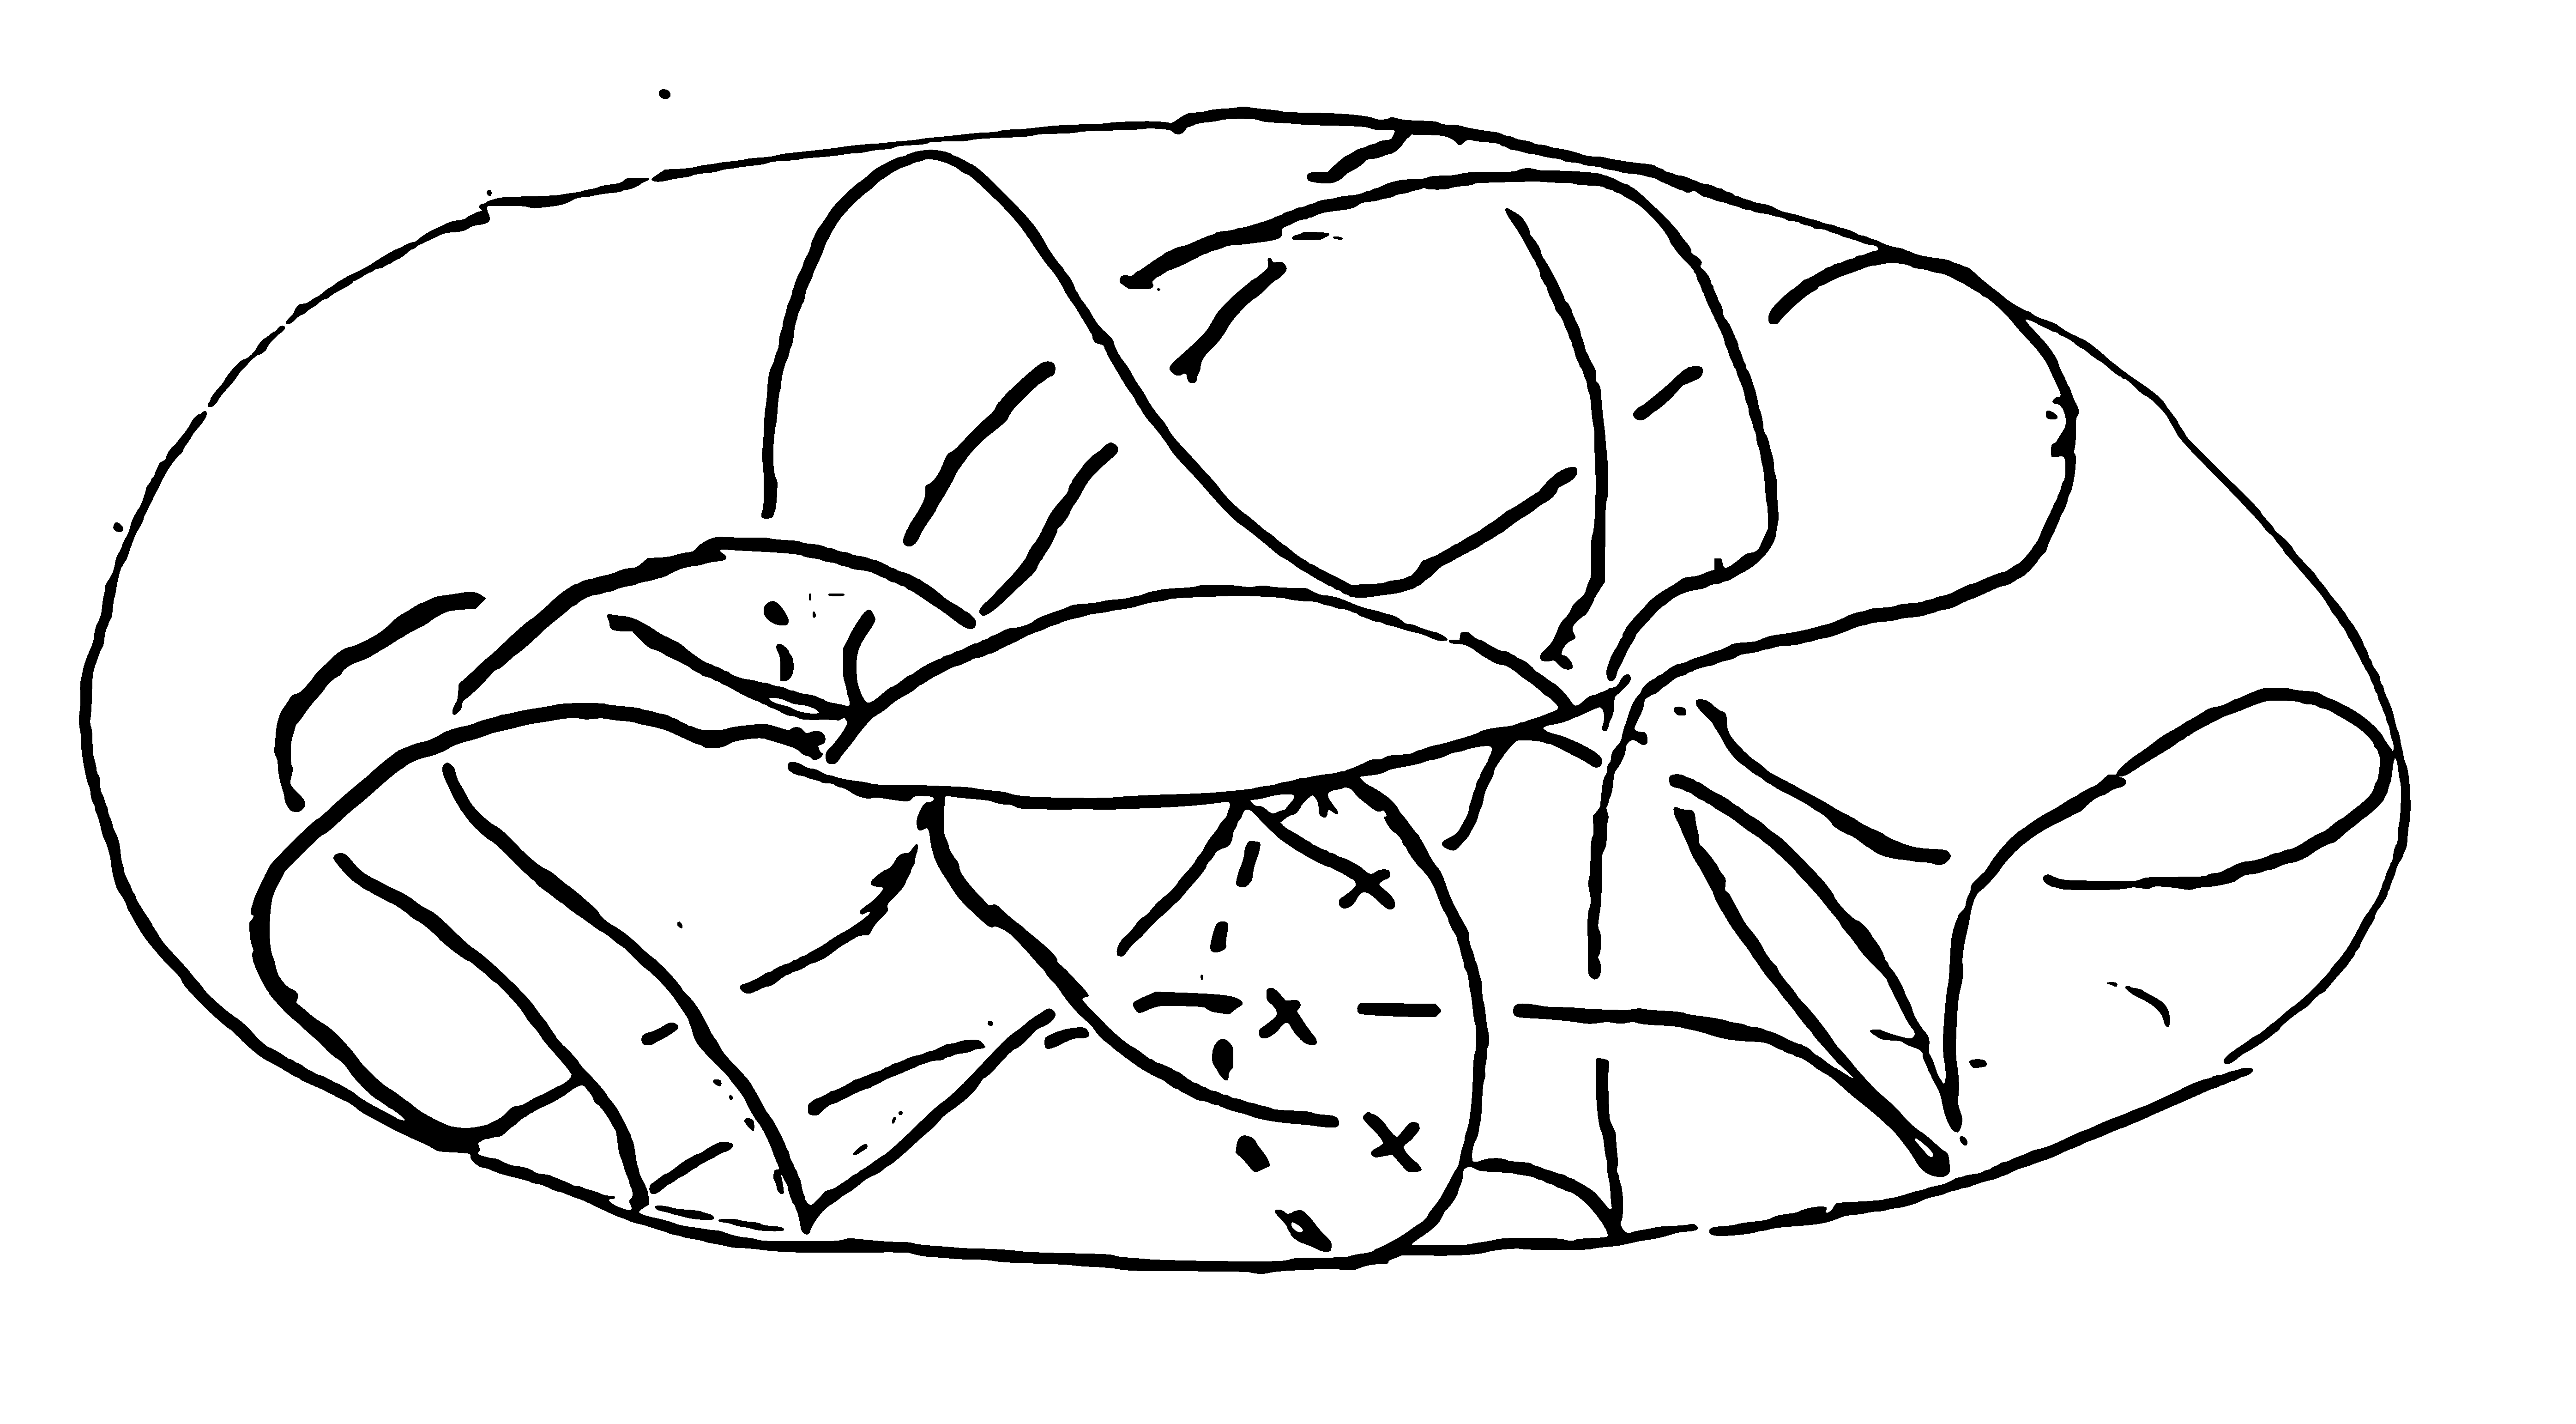
\includegraphics[width=0.5\textwidth]{figures/epätriviaali-torus-kuitukimppu.pdf}
    \caption{Epätriviaali torus, jossa kuidut ovat vääntyneitä.}
    \label{kuva:epätriviaali-torus-kuitukimppu}
\end{figure}
\begin{maaritelma}[Vektorikimppu]
    Olkoon $M$ topologinen avaruus. Asteen $k$ $\K$-\emph{vektorikimppu} $M$:n yli on jatkuvalla surjektiolla $\pi:E\to M$ varustettu topologinen avaruus $E$ siten, että 
    \begin{enumerate}
        \item kaikille $p\in M$ kuitu $E_p=\pi^{-1}(p)$ yli $p$:n voidaan varustaa $k$-ulotteisen $\K$-vektoriavaruuden rakenteella ja
        \item kaikille $p\in M$ on olemassa $p$:n ympäristö $U\subset M$ ja homeomorfismi $\Phi:\pi^{-1}(U)\to U\times\K^k$ siten, että
        \begin{itemize}
            \item $\pi_U\circ\Phi=\pi$ (jossa $\pi_U:U\times\K^k\to U$ on projektio) ja
            \item kaikille $q\in U$ $\Phi|_{E_q}$ on vektoriavaruusisomorfia $E_q\cong\{q\}\times\K^k\cong\K^k$.
        \end{itemize}
    \end{enumerate}
\end{maaritelma}
\begin{esimerkki}
    Esimerkiksi pallo ja sen tangenttikimppu muodostavat vektorikimpun $\pi:T\S^2\to\S^2$, jossa projektio määritetään $T_p\S^2\mapsto p$ eli pisteeseen, jossa tangenttiavaruus kiinnittyy palloon. Tässä jokainen kuitu voidaan varustaa 2-ulotteisella $\R$-rakenteella.
\end{esimerkki}
Pallo ja tangenttikimppu ovat esimerkkeji globaalisti triviaalista vektorikimpusta, jossa ei ole vääntöä. Möbius-nauha kuvassa~\ref{kuva:mobius-nauha} muistuttaa paikallisesti tuloa $\S^1\times I$, missä $I\subset\R$, mutta globaalisti se on vääntynyt.
\begin{figure}
    \centering
    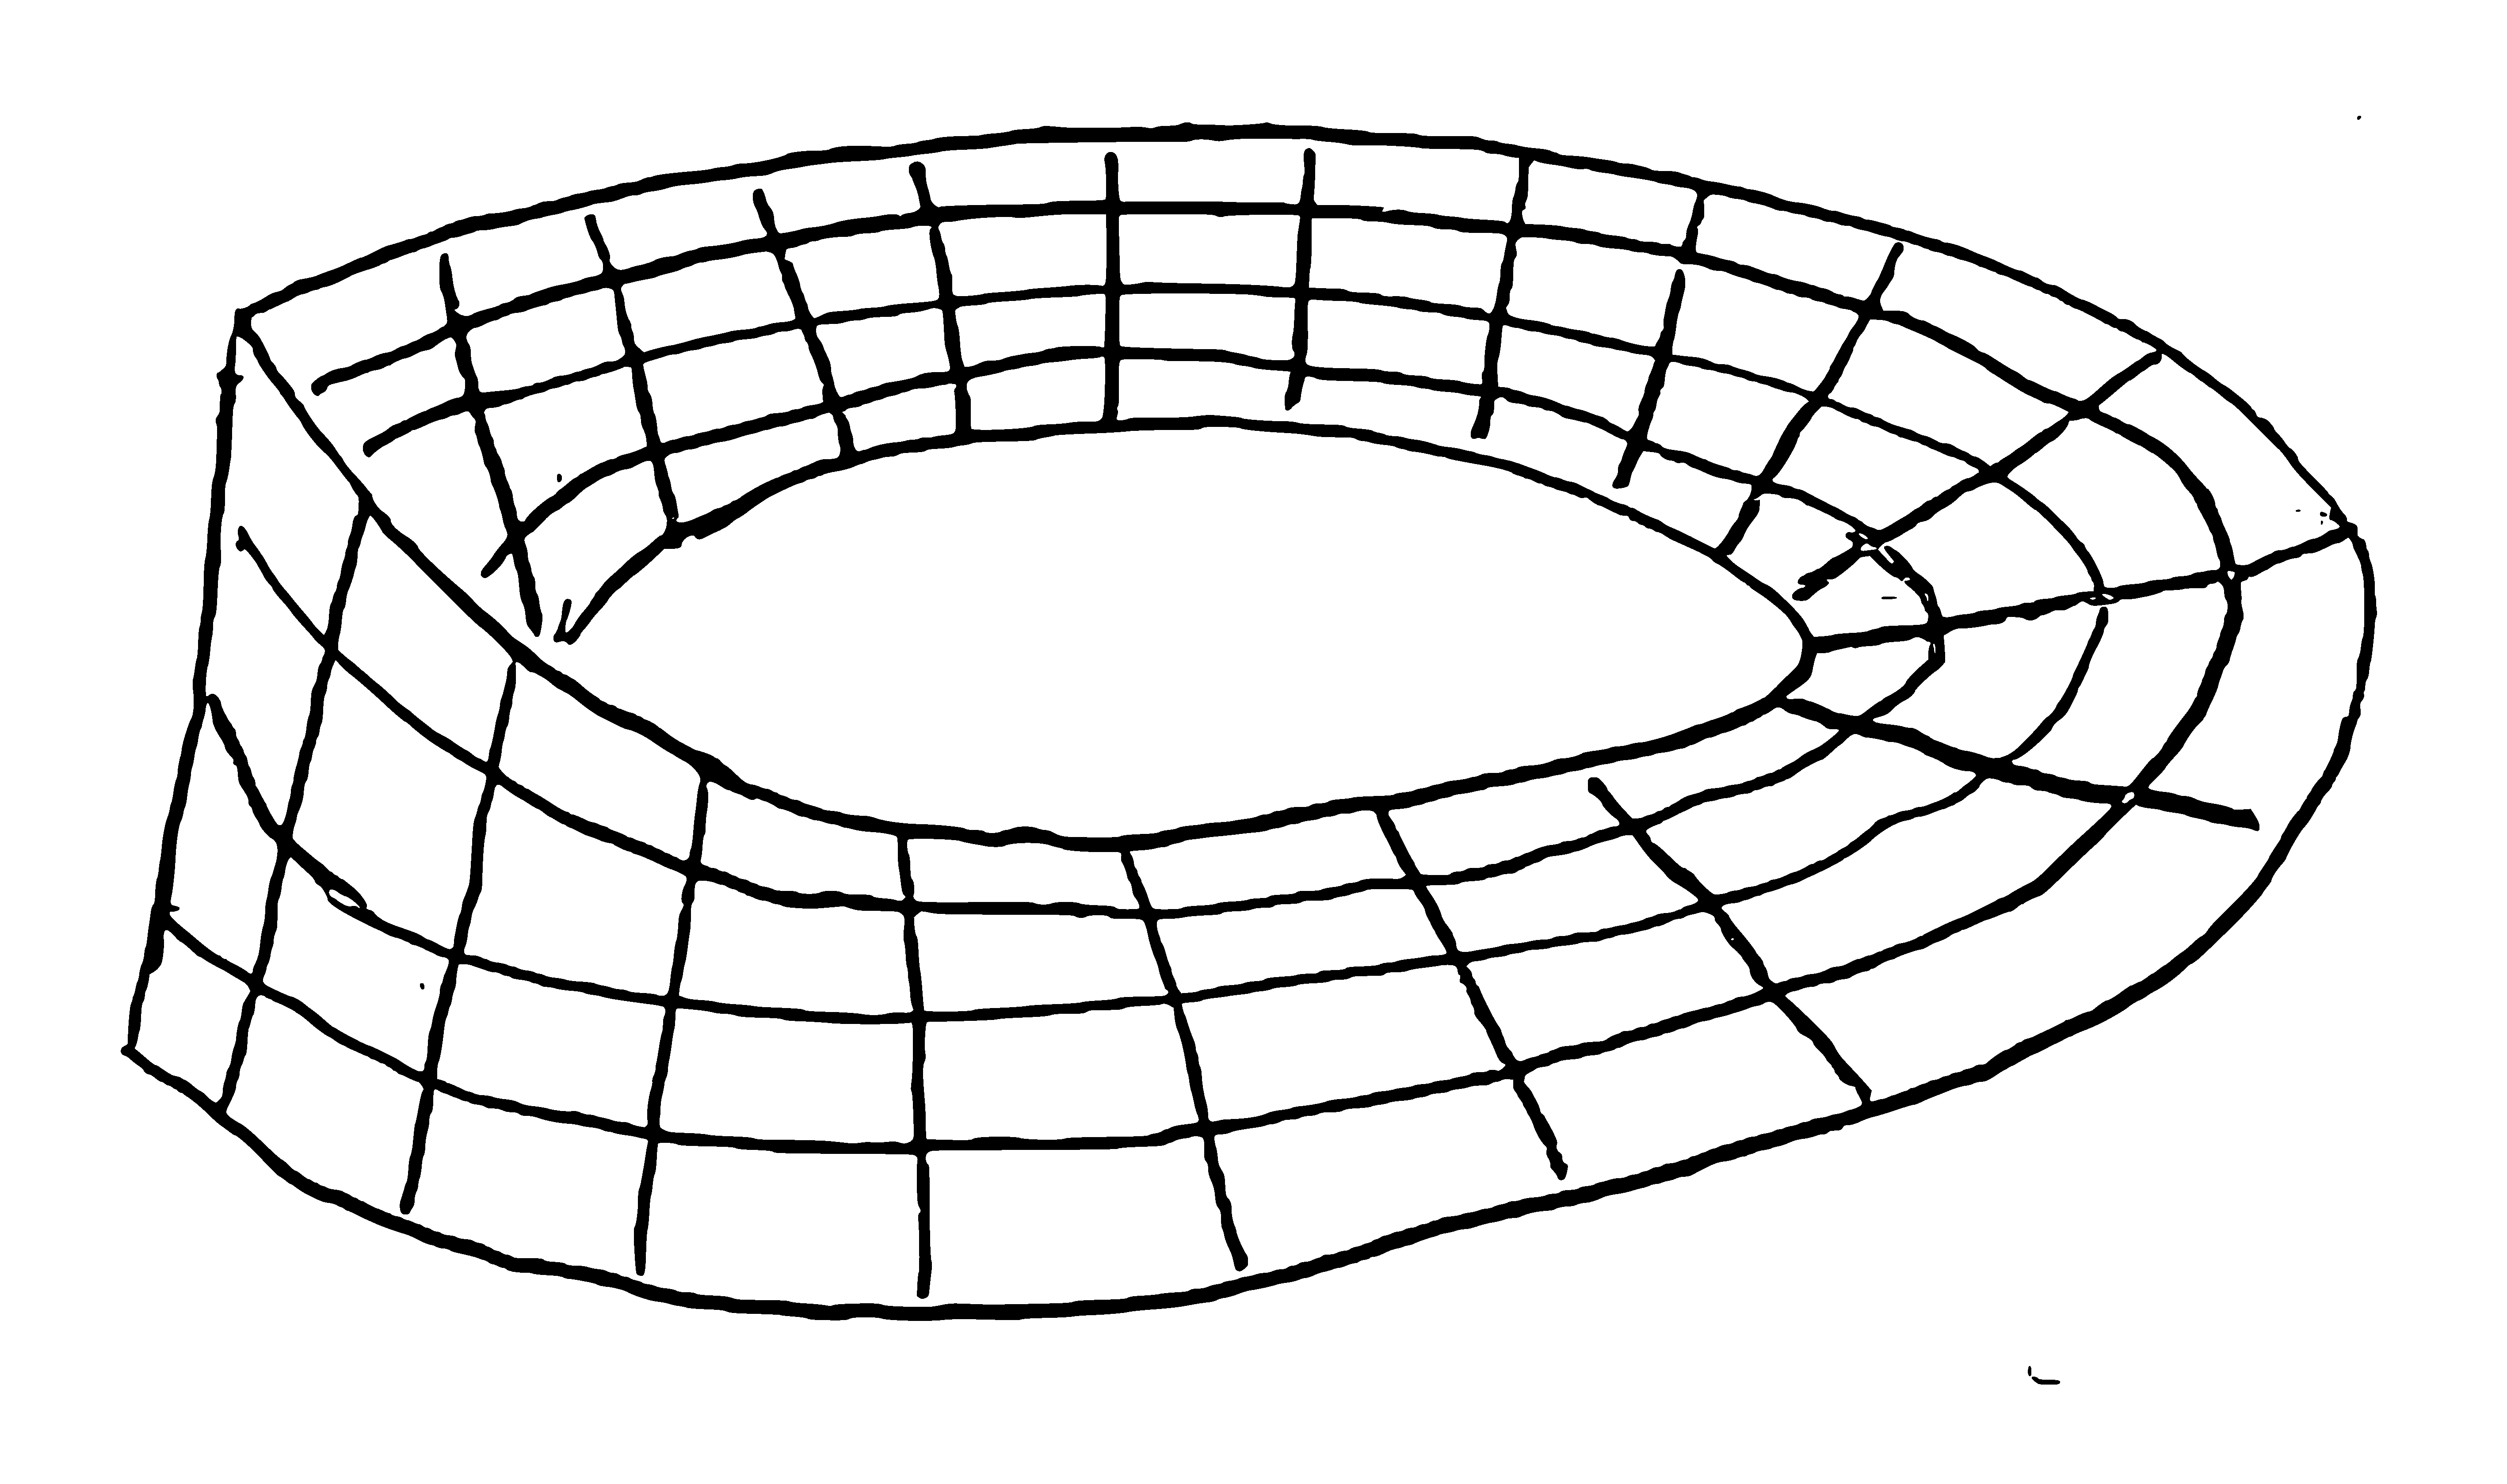
\includegraphics[width=0.5\textwidth]{figures/mobius-nauha.pdf}
    \caption{Möbius-nauha.}
    \label{kuva:mobius-nauha}
\end{figure}


\subsection{Kuidut}
Siinä missä kuitukimppu yleistää topologisen tulon, kuidutus yleistää kuitukimpun. Kuidutuskonstruktio on hankala käsittää ja se esitetään tässä pääosin vain myöhempää konstruktiota, putkiympäristöä, varten.
\begin{maaritelma}[Homotopinen nosto-ominaisuus]
    Kuvaus $\pi:E\to B$ tyydyttää \emph{homotopisen nosto-ominaisuuden} avaruudelle $X$, jos
    \begin{itemize}
        \item kaikille homotopioille $g:X\times[0,1]\to B$ ja
        \item kaikille kuvauksille $\tilde g_0:X\to E$ nostaen $g_0=g(\cdot,0)$:n, eli $p\circ\tilde g_0=g_0$,
    \end{itemize}
    on olemassa homotopia $\tilde g:X\times[0,1]\to E$ nostaen $g$:n (eli $g=p\circ\tilde g$) niin, että $\tilde g_0=\tilde g|_{X\times\{0\}}$. Kommutoiva kaavio havainnollistaa tilanteen:
    \begin{equation}
        \begin{tikzcd}
            X\times\{0\} \arrow[r, "\tilde g_0"] \arrow[d, hook] & E \arrow[d, "\pi"] \\
            X\times[0,1] \arrow[ur, dashrightarrow, "\tilde g"] \arrow[r, "g"] & B
        \end{tikzcd}
    \end{equation}
\end{maaritelma}
\begin{maaritelma}
    \emph{Kuidutus} on kuvaus $\pi:E\to B$, jolla on homotopinen nosto-ominaisuus kaikkien avaruuksien $X$ suhteen.
\end{maaritelma}
\begin{maaritelma}
    Olkoon $\pi:E\to B$ kuidutus. Kuidutus on \emph{paikallisesti triviaali}, jos kaikille $x\in B$ on olemassa avoin ympäristö $U\subset B$ siten, että 
    \begin{equation*}
        \pi^{-1}(U)\approx U\times F.
    \end{equation*}
\end{maaritelma}
\begin{maaritelma}
    Jos $E$ on pohja-avaruuden $B$ kuitukimppu $\pi:E\to B$, niin \emph{kuitukimpun sektio} on jatkuva kuvaus $\sigma:B\to E$ siten, että $\pi\circ\sigma=\text{id}_B$.
\end{maaritelma}

\subsection{Putket}
\begin{maaritelma}
    Olkoot $S,M$: $S\subset M$ sileitä monistoja. $S$:n \emph{putkiympäristö} $M$:ssä on pari $(\pi, J)$, jossa $\pi: E\to S$ on vektorikimppu ja $J:E\to M$ on sileä kuvaus, siten että
    \begin{itemize}
        \item $J\circ0_E=i$, $i$ on upotus $S\hookrightarrow M$ ja $0_E$ nollasektio
        \item on olemassa avoimet joukot $U\subset E$, $V\subset M$ siten, että $0_E[S]\subset U$ ja $S\subset V$ niin, että rajoitus $J|_U$ on diffeomorfismi.
    \end{itemize}
\end{maaritelma}
Yksinkertainen esimerkki saadaan käyrästä $\R^3$:ssa. Sen putkiympäristö on käyrää seuraileva kolmiulotteinen mato, jonka poikkileikkaukset ovat tasojoukkoja, joiden muoto vaihtelee, mutta käyrän suuntaisesti aina sileästi. Putkiympäristön läpileikkaus ei välttämättä ole ympyrälevyn mallinen. Esimerkki kuvassa~\ref{kuva:putkiympäristö}.
\begin{figure}
    \centering
    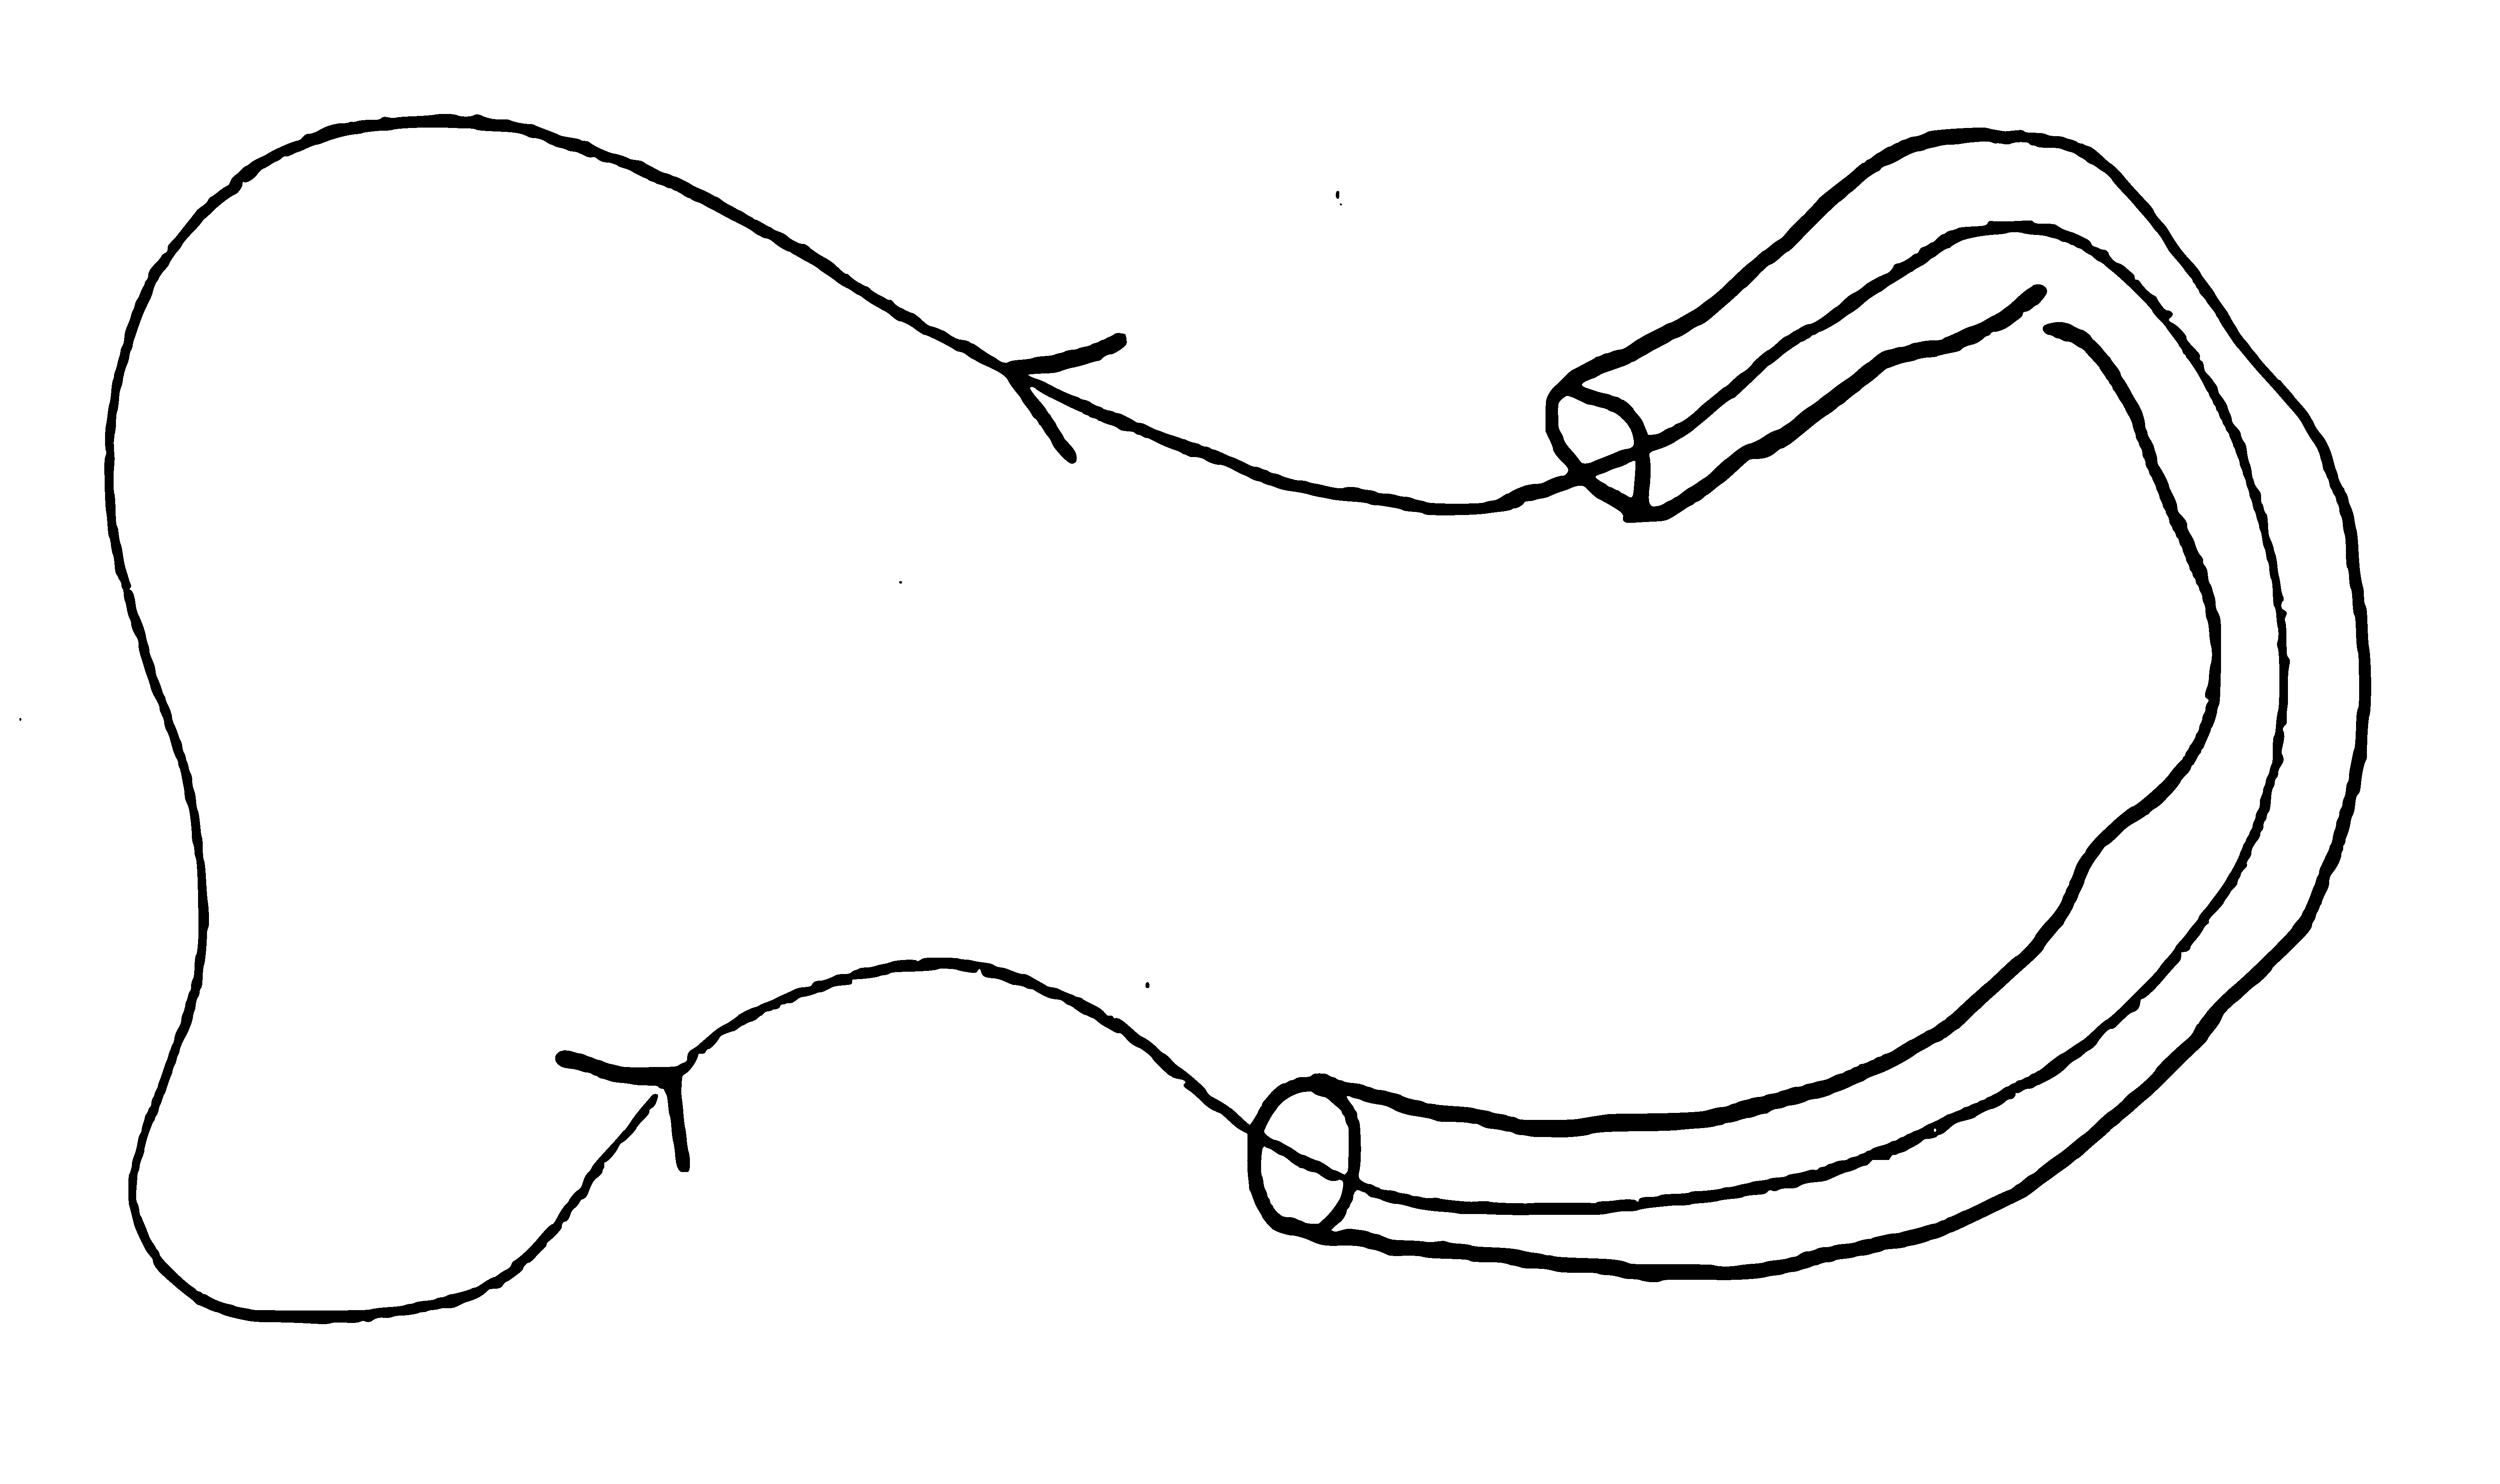
\includegraphics[width=0.5\textwidth]{figures/putkiympäristö.pdf}
    \caption{3-monistoon upotettu suljettu käyrä, jolle piirretty pätkä mielivaltaista putkiympäristöä.}
    \label{kuva:putkiympäristö}
\end{figure}
\begin{lause}[Putkiympäristölause]
    Jokaisella sileän moniston upotetulla sileällä alimonistolla on putkiympäristö.
\end{lause}
\begin{proof}
    Todistus on vaikea ja löytyy lähteestä ???.
\end{proof}
\begin{maaritelma}
    Olkoon $f:\C^2\to\C$ polynomikuvaus. Sen kuitua $f^{-1}(c),c\in\C$ kutsutaan \emph{säännölliseksi}, mikäli jollekin $c$:n ympärisölle $D$ kuvaus $f|_{f^{-1}(D)}:f^{-1}(D)\to D$ on paikallisesti triviaali $C^\infty$-kuidutus.

    Kuitu $f^{-1}(c)$ on \emph{säännöllinen äärettömyydessä}, jos jollekin $c$:n ympäristölle $E$ ja kompaktille osajoukolle $K\subset\C^2$ kuvaus $f|_{f^{-1}(D)-K}$ on paikallisesti triviaali kuidutus. 

    Jos kaikki $f$:n kuidut ovat säännöllisiä äärettömyydessä niin $f$ on \emph{hyvä}.
\end{maaritelma}
\begin{huomautus}
    ``Säännöllinen'' ja ``säännöllinen äärettömyydessä ja epäsingulaarinen'' ovat yhtäpitäviä.
\end{huomautus}
\begin{ajatus}
    Säännöllisyys on matemaattinen muotoilu idealle, että läheiset kuidut ``näyttävät samalta'' kuin $f^{-1}(c)$. Säännöllisyys äärettömyydessä muotoilee tämän samalta näyttämisen äärettömyyden ``lähellä''.
\end{ajatus}

\subsection{Homologiaa pintapuolisesti}
Homologia on sisällöltään rikas ja tekninen matematiikan osa-alue, jonka tarkoituksena on tutkia topologisten avaruuksien rakennetta ja reikiä. Homologian ehtisi tässä työssä esitellä vain lyhyesti, mikä ei tee aihepiirille oikeutta syvyytensä vuoksi; siispä aiheen esittely ohitetaan tässä työssä, mutta kiinnostunutta lukijaa ohjataan tutustumaan erinomaiseen Hatcherin materiaaliin \citep{Hatcher2002}.

Tässä aliosiossa esitetään kuitenkin lyhyt motivaatio homologialle sekä määritellään pari työssä keskeistä käsitettä. Määritelmät tarjoillaan intuitivistisen selityksen kera, homologiaa tuntematonta lukijaa silmälläpitäen.
\begin{ajatus}
    Homologia tutkii topologisten avaruuksien \emph{erilaisuutta} avaruuksien \emph{reikäisyyden} kautta. Reikäisyys on yllättävän vaikeaa määritellä, mutta se auttaa myös yllättävän hyvin erottelemaan avaruuksia toisistaan, esimerkiksi pallon ja toruksen.
\end{ajatus}
\begin{esimerkki}
    Ympyrä $\S^1$ ja kahdeksikko eivät ole homologisia. Ympyrällä sulkee sisäänsä yhden reiän, kahdeksikko kaksi reikää.
\end{esimerkki}
Ympyrän sisäänsä sulkema reikä on tietyssä mielessä kaksiulotteinen. Sitä rajaa yksiulotteinen ympyrä, ja sen paikalle voisi piirtää 2-pinnan. Samaan tapaan on olemassa kolmiulotteisia reikiä. Tällaisen sulkee sisäänsä $\S^2$. Tähän reikään ei voi päästä kolmiulotteisessa avaruudessa käsiksi kulkematta $\S^2$:n pinnan läpi, mutta neljättä ulottuvuutta pitkin reiän läpi voi kulkea koskematta $\S^2$:een.

Käytännössä homologiassa lasketaan homologiaryhmiä $H_n(X)$, missä $X$ on topologinen avaruus. Alaindeksi $n$ kertoo, että kyseessä on $n$:s homologiaryhmä, joka tavallaan mittaa avaruuden $n$-ulotteisia reikiä.
\begin{esimerkki}
    Ympyrälle $\S^1$ homologiaryhmät ovat
    \begin{equation*}
        H_i(\S^1)=
        \begin{cases}
            \Z, & i=0,1 \\
            0, & i>1
        \end{cases}.
    \end{equation*}
    Nollas homologiaryhmä $H_0$ mittaa avaruuden yhtenäisten komponenttien määrää. $H_0(\S^1)=\Z$ tarkoittaa, että ympyröitä voisi olla $k$ kappaletta liimattuna päällekkäin, $k\in\Z$ tai nolla, jos $k=0$.

    $H_1$ mittaa 1-ulotteisten reikien määrää, sitä, montako silmukkaa avaruus tekee yksiulotteisesti.

    $H_n$ mittaa $n$-ulotteisten reikien määrää, mutta $\S^1$:llä ei ole $n$-ulotteisia reikiä.
\end{esimerkki}
\begin{esimerkki}
    Pallon $\S^2$ tapauksessa $H_2(\S^2)=\Z$, mutta $H_1(\S^2)=0$, koska pallon pinnalle piirretyn ympyrän voi aina kiristää pisteeksi, mutta pinnalle asetettua huppua ei voi.
\end{esimerkki}
\begin{esimerkki}
    Toruksella $\T^2=\S^1\times\S^1$ on mielenkiintoisempia ryhmiä:
    \begin{equation*}
        H_i(\T^2)=
        \begin{cases}
            \Z, & i=0,2 \\
            \Z\oplus\Z, & i=1 \\
            0, & i>2
        \end{cases}
    \end{equation*}
    Ryhmä $H_1$ selittyy sillä, että toruksen pinnalle voi piirtää kaksi silmukkaa, joita ei voida muuntaa toisikseen: toruksen ison akselin ympäri, sekä toruksen paksuutta pitkin. Tämä on havainnollistettu kuvassa~\ref{kuva:toruksen-homologia-akselit}
\end{esimerkki}
\begin{figure}
    \centering
    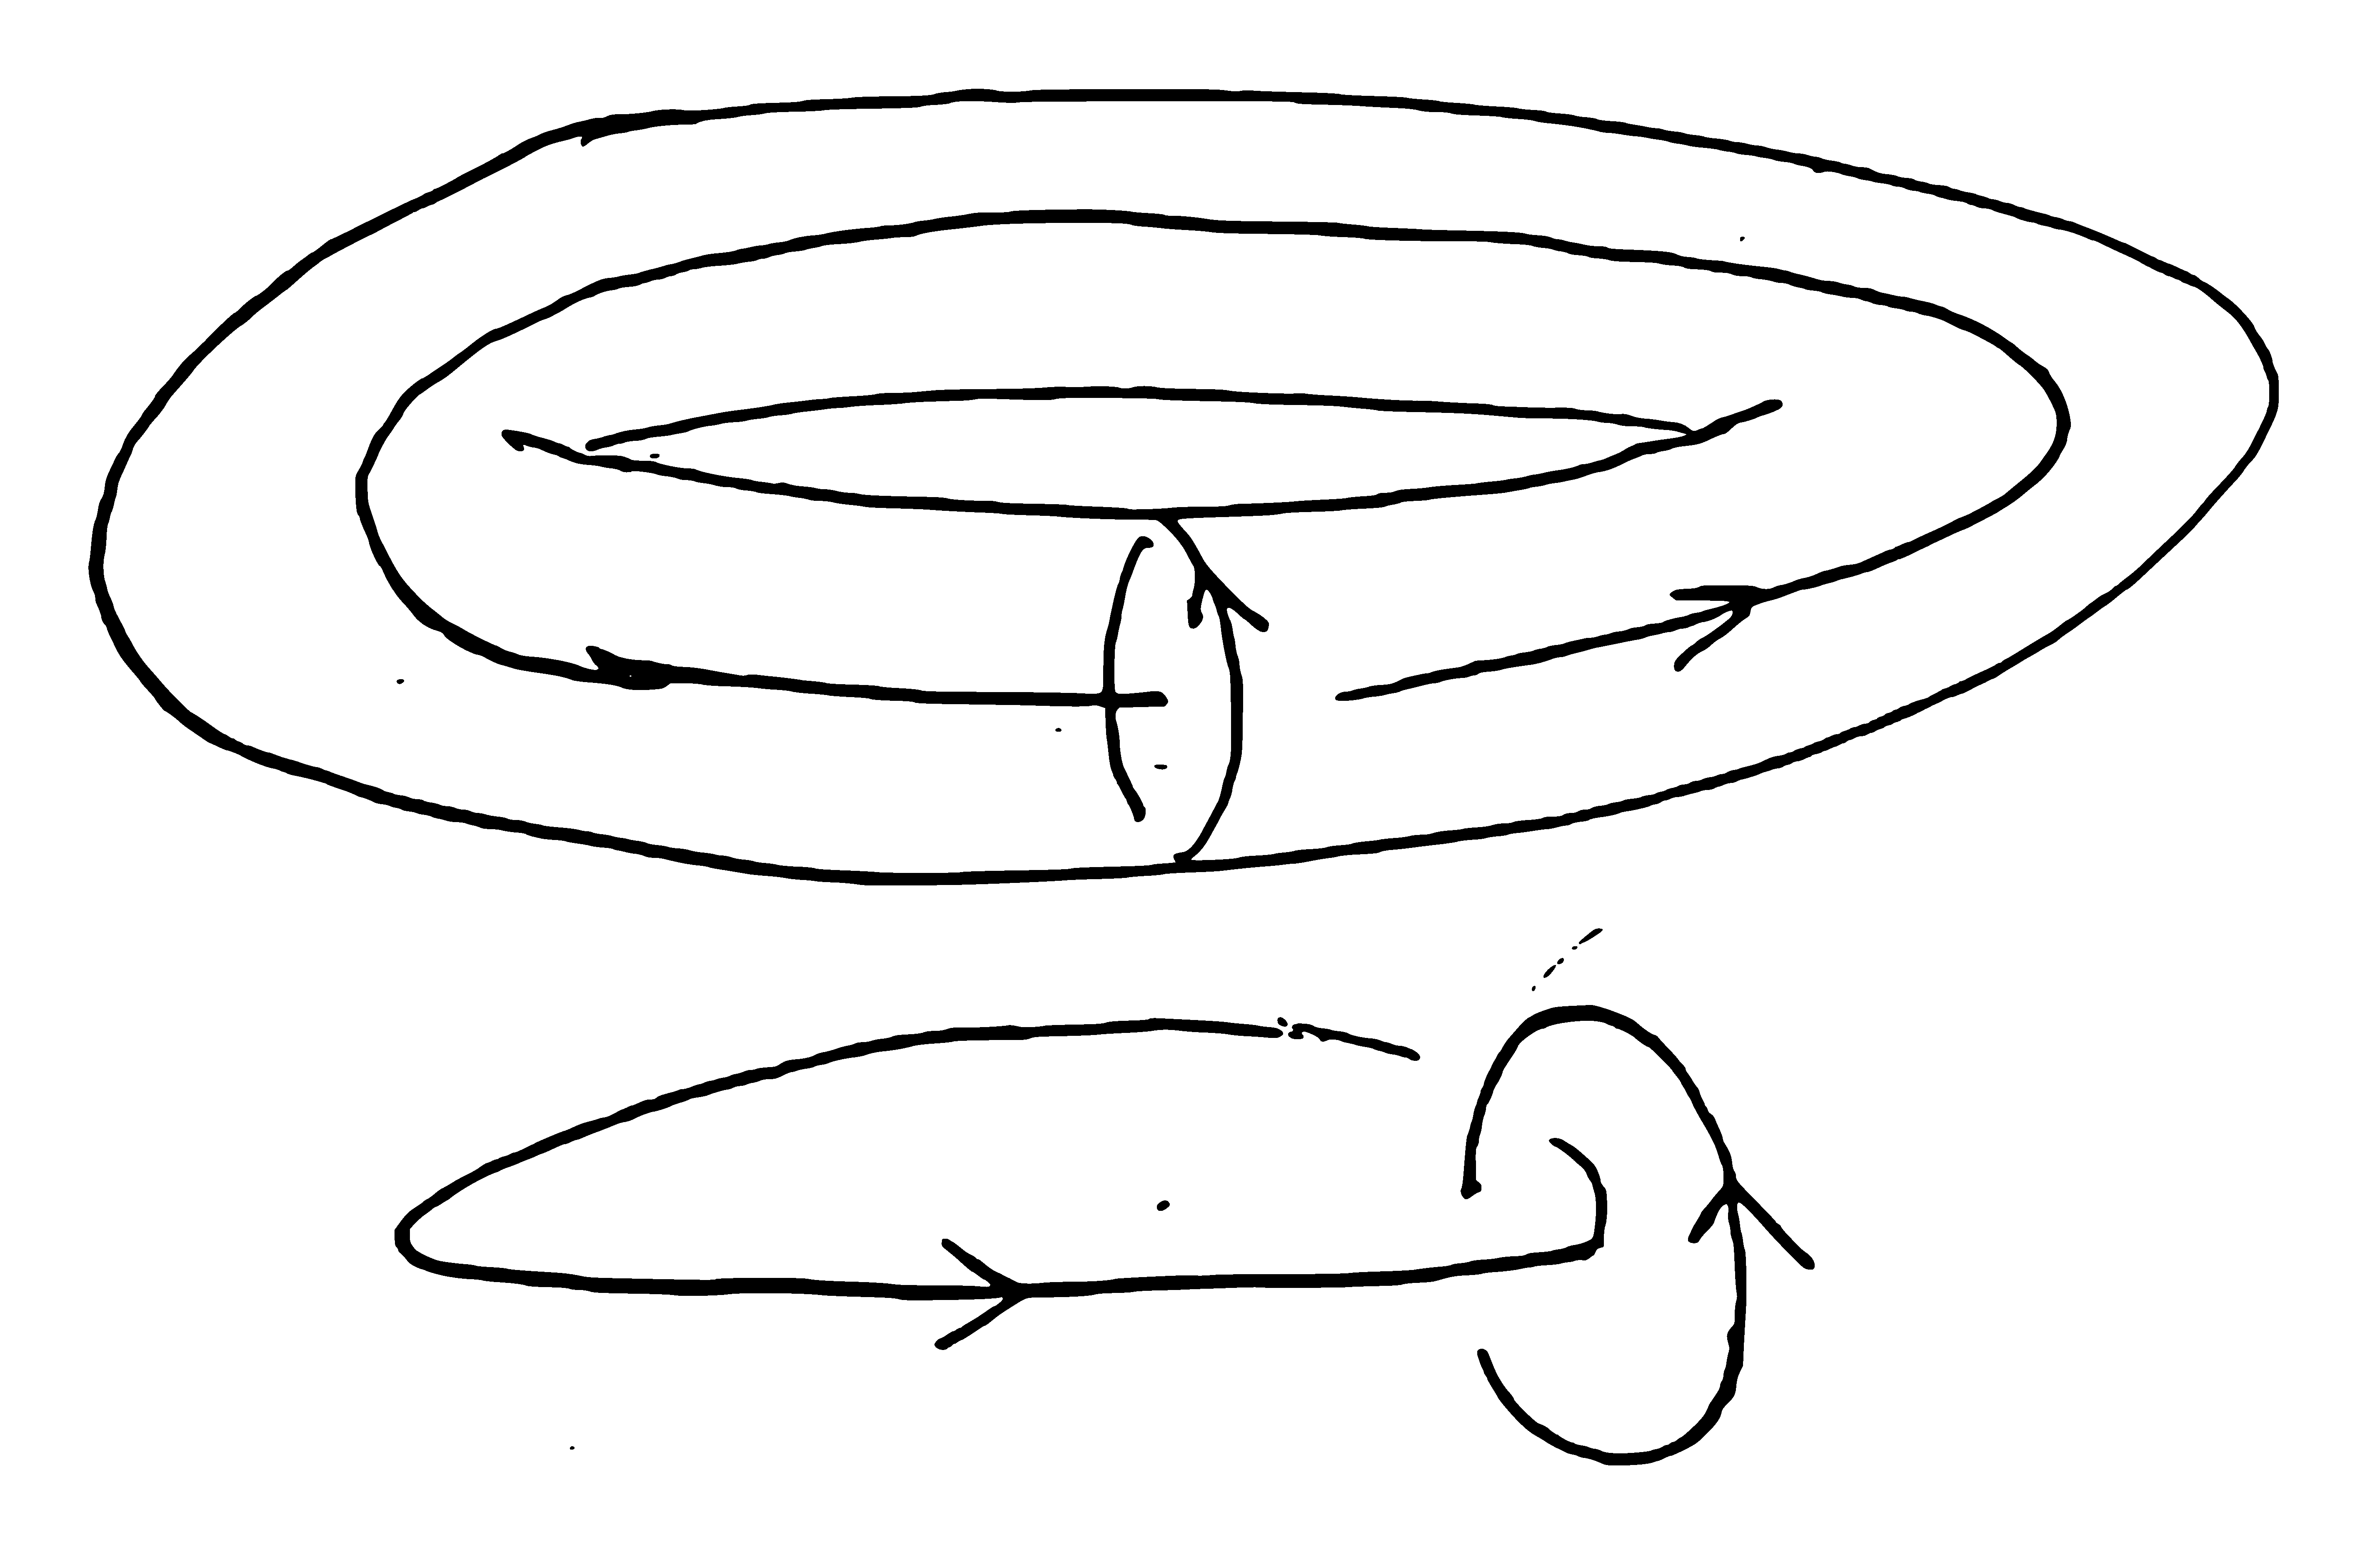
\includegraphics[width=0.5\textwidth]{figures/toruksen-homologia-akselit.pdf}
    \caption{Toruksen kaksi homologia-akselia.}
    \label{kuva:toruksen-homologia-akselit}
\end{figure}
Mitä ympyröiden homologiaryhmiin tulee, lukija saattoi huomata jo kaavaan, joka todistetaan lemmassa~\ref{lemma:ympyröiden-homologia}.
\begin{lemma}
    \label{lemma:ympyröiden-homologia}
    Kaikille $n$-palloille $\S^n$ pätee
    \begin{align*}
        H_0(\S^n)&=H_n(\S^n)=\Z, \\
        H_k(\S^n)&=0,\quad k\ne n.
    \end{align*}
\end{lemma}
\begin{proof}
    Mayer-Vietoris-jono.
\end{proof}
Homologia ei ole kuitenkaan täydellinen keino topologisten avaruuksien erottelemiseksi. On olemassa avaruuksia, jotka eivät ole homeomorfisia, vaikka niiden homologiaryhmät ovat samat kaikilla $n\in\N_0$. Työn kannalta tärkeä yleinen avaruus, jossa työskennellään paljon, on avaruus, joka ainakin homologisesti muistuttaa palloa.
\begin{maaritelma}
    \label{maar:homologinen-n-pallo}
    Topologinen $n$-monisto $X$ on \emph{homologinen $n$-pallo}, jos se tyydyttää lemman~\ref{lemma:ympyröiden-homologia} yhtälöt, ts.
    \begin{align*}
        H_0(X)&=H_n(X)=\Z \\
        H_k(X)&=0,\quad k\ne n
    \end{align*}
\end{maaritelma}

\subsection{Kuidutetut torukset}
Ok ilmeisesti kuidutetut torukset on aika tärkee juttu ja kuidutetut Seifert-monistot (avaruudet?) myös. Tähän tulis selitystä niistä.

\subsection{Homologia (aksiomaattinen yritys)}
Tämä on vähän epätoivoinen yritys sisällyttää homologia työhön. Taidan poistaa koko osion.

Tämän aliosion tarkoitus on kiinnittää työssä käytettävä homologian sanasto. Työn tiivis esitys ei tee oikeutta homologialle ja homologiaa tuntematonta lukijaa suositellaankin sivuuttamaan osio, tai tutustumaan homologiaan Hatcherin kirjan avulla \citep{Hatcher2002}. Aliosio on pikemminkin suunnattu homologiaa tuntevalle lukijalle, joka haluaa varmistaa termistön, tai palata työn myöhemmistä osioista tarkistamaan määritelmiä. Sanastossa noudatetaan kuitenkin yleisiä tapoja, joten myös homologiaa tunteva lukija voi sivuuttaa aliosion.
\begin{maaritelma}
    \emph{CW-kompleksi} on topologinen avaruus $X$, joka muodostetaan algoritmisesti:
    \begin{enumerate}
        \item Valitaan diskreetti joukko $X^0$, jonka alkioita kutsutaan $X$:n \emph{$0$-soluiksi}.
        \item Muodostetaan induktiivisesti \emph{$n$-luuranko $X^n$} $X^{n-1}$:stä liittämällä $n$-soluja $e_\alpha^n$ kuvauksilla $\varphi_\alpha:\pallo^{n-1}\to X^{n-1}$. $X^n$ on tekijä-avaruus
        \begin{equation}
            X^n=\frac{X^{n-1}\sqcup_\alpha D_\alpha^n}{\sim},
        \end{equation}
        missä $\sim$ on relaatio $x\sim\varphi_\alpha(x)$, kun $x\in\partial D_\alpha^n$. Joukon $D_\alpha^n-\partial D_\alpha^n$ kuva tekijäkuvauksen suhteen ja solu $e_\alpha^n$ ja ovat homeomorfisia.
        \item Jatkamalla prosessia saadaan $X=\cup_n X^n$ ja se voidaan varustaa heikolla topologialla: $A\subset X$ on avoin (suljettu) jos ja vain jos $A\cap X^n$ on avoin (suljettu) $X^n$:ssä kaikille $n\in\N$. 
    \end{enumerate}
\end{maaritelma}
\begin{aksiooma}[Homologia-aksioomat]
    \begin{enumerate}
        \item Jos $f\cong g:X\to Y$ niin $f_\bullet=g_\bullet:\tilde h_n(X)\to\tilde h_n(Y)$.
        \item On olemassa reunahomomorfismit $\partial:\tilde h_n(X/A)\to\tilde h_{n-1}(A)$ määritelty kaikille CW-pareille $(X,A)$, siten että jono
        \begin{equation}
            \cdots\xrightarrow{\partial}\tilde h_n(A)\xrightarrow{i_\bullet}\xrightarrow{q_\bullet}\tilde h_n(X/A)\xrightarrow{\partial}\tilde h_n(A)\xrightarrow{i_\bullet}\cdots
        \end{equation}
        on tarkka. Jonossa $i$ on inkluusio ja $q$ tekijäkuvaus.
    \end{enumerate}
\end{aksiooma}
\begin{maaritelma}
    Pelkistetty homologiateoria antaa epätyhjille CW-komplekseille $X$ jonon
    \begin{itemize}
        \item abelisia ryhmiä $\tilde h_n(X)$ ja
        \item homomorfismeja $f_\bullet:\tilde h_n(X)\to\tilde h_n(Y)$ jokaista CW-kompleksien välistä kuvausta $f:X\to Y$ kohden, siten että
        \begin{itemize}
            \item $(fg)_\bullet=f_\bullet g_\bullet$
            \item $\mathbbm{1}_\bullet=\mathbbm{1}$,
        \end{itemize}
    \end{itemize}
    siten, että homologia-aksioomat pitävät.
\end{maaritelma}
\section{Algebralliset käyrät ja projektiiviset avaruudet}
Tämän osion tarkoituksena on esitellä tiiviisti algebrallisten käyrien, projektiivisten avaruuksien ja projektiivisten käyrien määritelmän sanaston kiinnittämiseksi. Kiinnostunut lukija löytää huolellisemman tarkastelun esimerkiksi Gathmannin algebrallisen geometrian luentomuistiinpanoista \citep{gathmann-ag}.

\subsection{Affiinit algebralliset käyrät kompleksitasossa}
Affiini algebrallinen käyrä kompleksitasossa on määritelty polynomin nollakohtien joukkona. Tarkemmin sanottuna, jos $f \in \mathbb{C}[x,y]$ on ei-vakio polynomi, niin affiini algebrallinen käyrä $C$ joka liittyy polynomiin $f$ on joukko
\begin{equation}
    C = \{ (x,y) \in \mathbb{C}^2 \mid f(x,y) = 0 \}.
\end{equation}
Koska $\C$ on algebrallisesti suljettu, niin jokainen polynomi $f \in \mathbb{C}[x,y]$ voidaan tekijöidä lineaarisiin tekijöihin. Tämän vuoksi jokainen affiini algebrallinen käyrä kompleksitasossa voidaan esittää lineaaristen käyrien yhdistelmänä.

\subsection{Singulariteetit ja säännöllisyys}
Käyrän $C$ paikallisen muodon pisteessä $p=(a,b)\in C$ määrittyy $f$:n osittaisderivaattojen avulla. Piste $p$ on \emph{singulaarinen} (tai kriittinen), jos $f$:n osittaisderivaatat häviävät pisteessä $p$:
\begin{equation}
    \frac{\partial f}{\partial x}(a,b) = 0 \quad \text{ja} \quad \frac{\partial f}{\partial y}(a,b) = 0
\end{equation}
Jos vähintään yksi osittaisderivaatoista ei ole nolla $p$:ssä, niin piste on \emph{säännöllinen}. Säännöllisessä pisteessä implisiittisten funktioiden lause takaa, että käyrä näyttää paikallisesti kompleksisen 1-ulotteiselta varistolta, ja on mahdollista määritellä yksikäsitteinen tangenttisuora.

\subsection{Projektiivinen taso ja suora}
Affiinilla avaruudella $\C$ on geometrinen rajoitus: kaksi erillistä suoraa leikkaavat yleensä yhdessä pisteessä, paitsi jos ne ovat yhdensuuntaisia. Yhtenäistääksemme näitä geometrisia käsitteitä, otamme käyttöön projektiivisen avaruuden.

Kompleksinen $n$-ulotteinen projektiivinen avaruus $\P^n(\C)$ määritelläänjoukoksi, joka koostuu avaruuden $\C^{n+1}$ vektorisäteistä (tai niiden ekvivalenssiluokista), jotka kulkevat origon kautta. Toisin sanoen, $\P^n(\C)$ on määritelty seuraavasti:
\begin{maaritelma}
    Olkoon $(Z_0,\dots,Z_n) \in \C^{n+1} \setminus \{0\}$. Määritellään ekvivalenssirelaatio $\sim$ seuraavasti:
    \begin{equation*}
        (Z_0,\dots,Z_n) \sim (\lambda Z_0, \dots, \lambda Z_n) \quad \text{kaikille } \lambda \in \C^*.
    \end{equation*}
    Tällöin
    \begin{equation*}
        \P^n(\C):=\frac{\C^{n+1}\setminus\{0\}}{\sim}.
    \end{equation*}
    Ekvivalenssiluokan edustaja merkitään homogeenisilla koordinaateilla $[Z_0:\dots:Z_n]$.
\end{maaritelma}
\begin{asetus}
    Jatkossa merkitään $\P^n$ pidemmän $\P^n(\C)$ sijasta, koska tässä työssä keskitytään yksinomaan kompleksisten käyrien tarkasteluun.
\end{asetus}
\begin{esimerkki}
    \label{esim:proj-taso-ja-suora}
    Tapauksissa $n=1$ ja $n=2$
    \begin{itemize}
        \item $\P^1\cong\C\cup\{\infty\}$ (Riemann-pallo)
        \item $\P^2\cong\C^2\cup\P^1$. $\P^2$:n koordinaatit ovat $[X:Y:Z]$, ja $\P^1$ on joukko pisteitä, joilla $Z=0$.
    \end{itemize}
    Jos tarkastellaan projektiivisten avaruuksien ulottuvuuksia reaalimielessä ($\dim_\R(\C)=2$), niin $\dim_\R(\P^1)=2$ ja $\dim_\R(\P^2)=6$ (vai 4?).
\end{esimerkki}

\subsection{Upotus \texorpdfstring{$\C^2\hookrightarrow\P^2$}{Upotus C²→P²}}
\begin{lemma}
    \label{lemma:projektiivisen-avaruuden-jako}
    Projektiivinen avaruus on erillinen yhdiste $\P^{n}=\C^n\sqcup\P^{n-1}$.
\end{lemma}
\begin{proof}
    Tarkastellaan $\P^{n}$:n pistettä $[Z_0:\dots:Z_{n}]$, jolla on $n$ koordinaattia. Jos $Z_{n+1}\neq 0$, niin piste voidaan esittää muodossa
    \begin{equation*}
        [Z_0:\dots:Z_n] \sim [Z_0:\dots:Z_{n-1}:1] \in \C^n,
    \end{equation*}
    koska on olemassa $\lambda\in\C\setminus\{0\}$, jolla $\lambda Z_n=1$. Jos taas $Z_n=0$, niin piste kuuluu $\P^{n-1}$-joukkoon. Tällöin saadaan jako $\P^{n}=\C^n\sqcup\P^{n-1}$.
\end{proof}
Lemma yleistää esimerkin \ref{esim:proj-taso-ja-suora}: yleisen projektiivisen avaruuden $\P^n$ ``sisus'' on $\C^n$ ja ``kuori äärettömyydessä'' $\P^{n-1}$, joka induktiivisesti kuortaan lukuunottamatta muistuttaa $\C^{n-1}$:tä. Tämä antaa mielekkään upotuksen $\C^n\hookrightarrow\P^n$.

Työlle relevantissa 2-ulotteisessa tapauksessa avaruus $\C^2$ voidaan nähdä paikallisena karttana (tai tiheänä avoimena joukkona) projektiivisessa tasossa $\P^2(\C)$. Tyypillinen upotus määritellään seuraavasti:
\begin{equation}
    \begin{aligned}
        \iota : \C^2 &\hookrightarrow \P^2(\C) \\
        (x,y) &\mapsto [x : y : 1]
    \end{aligned}
\end{equation}
Pisteet $\P^2$:ssa, jotka eivät kuulu tämän upotuksen kuvaan, ovat muotoa $[X:Y:0]$. Näiden pisteiden joukko muodostaa projektiivisen suoran $\P^1$, jota kutsutaan \emph{suoraksi äärettömyydessä} tai \emph{äärettömyyssuoraksi}. Lemman \ref{lemma:projektiivisen-avaruuden-jako} hengessä $\P^2=\C^2\sqcup\P^1$.

\subsection{Projektiiviset käyrät}
Projektiivisessa tasossa $\P^2$ klassinen polynomi $f(x,y)$ ei ole hyvin määritelty, koska homogeeniset koordinaatit ovat ekvivalentteja skalaarikertoimen suhteen. Tämän vuoksi on käytettävä \emph{homogeenistä} polynomia $F(X,Y,Z)$, eli polynomia, jossa kaikilla monomeilla on sama aste $d$. Yhtälö $F(\lambda X, \lambda Y, \lambda Z) = \lambda^d F(X,Y,Z) = 0$ on tällöin riippumaton valitusta edustajasta.
\begin{maaritelma}[Homogenisointi]
    Polynomi $f(x,y) \in \C[x,y]$ voidaan \emph{homogenisoida} määrittelemällä
    \begin{equation}
        F(X,Y,Z) = Z^d f\left(\frac{X}{Z}, \frac{Y}{Z}\right),
    \end{equation}
    missä $d$ on polynomin $f$ aste.
\end{maaritelma}
\begin{maaritelma}
    Projektiivinen algebrallinen käyrä $\mathcal{C}$ määritellään homogeenisen polynomin $F(X,Y,Z)$ nollakohtien joukkona:
    \begin{equation}
        \mathcal{C} = \{ [X:Y:Z] \in \P^2 \mid F(X,Y,Z) = 0 \}.
    \end{equation}
\end{maaritelma}
\begin{huomautus}
    Polynomin homogenisointi sallii luonnollisesti käyrän tarkastelun myös äärettömyyssuoralla. Projektiivinen käyrä $\mathcal{C}$ on aina suljettu ja kompakti, koska se on suljettu alijoukko projektivisessa avaruudessa $\P^2$, joka on itsessään kompakti.
\end{huomautus}

\section{Solmut}

Matematiikassa solmuja tarkastellaan ympyrännäköisinä topologisina olioina, jotka saavat sotkeutua itseensä. Epämuodollisesti määriteltynä matemaattinen solmu on kuin tavallinen solmu, jonka päät on liimattu yhteen. Linkillä tarkoitetaan kappaletta, joka koostuu erillisistä solmuista, jotka voivat olla kietoutuneina toisiinsa. Työssä noudatetaan D. Eisenbudin ja W. D. Neumannin \citep{EN1985} merkintätapoja ja joitakin peruskäsitteitä lainataan Rolfsenin kirjasta \citep{Rolfsen1976}.
\begin{maaritelma}
    Topologisen avaruuden $X$ osajoukko $\solmu\subset X$ on \emph{solmu}, jos $\solmu$ on homeomorfinen palloon $\pallo^p$, jollekin $p\in\N$.
\end{maaritelma}
\begin{maaritelma}
    \emph{Linkki} $\linkki=(\Sigma,S_1\cup\cdots\cup S_n)$ on pari, jossa $\Sigma$ on suunnattu homologinen $n$-pallo ja $S_i$ on kokoelma sileitä, erillisiä, suunnattuja ja yksinkertaisia\footnote{Yksinkertainen käyrä ei leikkaa itseään.} käyriä $\Sigma$:ssa.
\end{maaritelma}
\begin{maaritelma}
    Linkkien $\linkki=(\Sigma,S_1\cup\cdots\cup S_n)$ ja $\linkki'=(\Sigma',S_1'\cup\cdots\cup S_m')$ \emph{erillinen summa} on
    \begin{equation*}
        \linkki+\linkki'=(\Sigma\#\Sigma',S_1\cup\cdots\cup S_n\cup S_1'\cup\cdots\cup S_m'),
    \end{equation*}
    jossa $\Sigma\#\Sigma'$ on $\Sigma$ ja $\Sigma'$:n yhtenäinen summa $S_i$:tä leikkaamattomien levyjen kautta. 
    
    Linkkien \emph{yhtenäinen summa} on
    \begin{equation*}
        \linkki\#\linkki'=(\Sigma\#\Sigma',(S_1\#S_1')\cup S_2\cup\cdots\cup S_n\cup S_2'\cup\cdots\cup S_m'),
    \end{equation*}
    jossa $\Sigma$:n ja $\Sigma'$:n yhtenäinen summa otetaan kautta levyjen, jotka leikkaavat linkkejä väleissä $I\subset S_1$ ja $I'\subset S_1'$.
\end{maaritelma}
\begin{maaritelma}
    Solmun $\solmu$ putkiympäristöä merkitään $N(\solmu)$ ja linkin $\linkki=(\Sigma,S_1\cup\cdots\cup S_n)$ putkiympäristö määritellään $N(\linkki):=N(S_1)\cup\cdots\cup N(S_n)$.
\end{maaritelma}
\begin{maaritelma}
    Linkin osasen $S_i$ pituuspiiri $M_i$ ja leveyspiiri $L_i$ ???
\end{maaritelma}
\begin{maaritelma}[Linkkien pujos]
    Olkoot $\linkki=(\Sigma,S_1\cup\cdots\cup S_n)$ ja $\linkki'=(\Sigma',S_1'\cup\cdots\cup S_m')$ linkkejä. Määritellään
    \begin{equation*}
        \Sigma''=(\Sigma-\interior N(S))\cup(\Sigma'-\interior N(S'))
    \end{equation*}
    liimaamalla avaruuksien reunat toisiinsa siten, että samansuuntaisesti päällekkäin liitetään $M$ ja $L'$ sekä $L$ ja $M'$. $\Sigma''$ on suunnattu homologinen 3-pallo [???]. Linkki
    \begin{equation*}
        \linkki''=(\Sigma'',(K-S)\cup(K'-S'))
    \end{equation*}
    on $\linkki$:n ja $\linkki'$:n \emph{pujos} ja sitä merkitään
    \begin{equation*}
        ??? kaavio ???:\ L-_S-_{S'}-L'
    \end{equation*}
\end{maaritelma}

\begin{maaritelma}
    \emph{Seifert-linkki} on linkki $\mathbf L=(\Sigma,K)=(\Sigma',\cup_{i=1}^n K_i)$, jonka ulkoreunalla $\Sigma_0=\Sigma'-\text{int } N(K)$ on Seifert-kuidutus.
\end{maaritelma}
\section{Pujoskaavio}
Solmuja voi pujoa peräkkäin useita ja monimutkaisilla tavoilla, jolloin solmujen piirtäminen käy nopeasti hyvin vaikeaksi. Monimutkaisten linkkien kuvaamiseen hyödyllinen työkalu ovat pujoskaaviot, jotka ovat tietynlaisia verkkoja. Verkko on matemaattinen olio, joka koostuu silmuista ja niitä yhdistävistä kaarista. Pujoskaavioissa kaariin liitetään kokonaislukukertoimet, jotka kertovat tietoa solmusta.

Pujoskaavioihin liittyy monta hankalaa ideaa, koska monimutkaisten linkkien esittäminen yksinkertaisesti, mutta yksiselitteisesti, on hyvin vaikeaa. Sen takia tässä kappaleessa pujoskaavioiden rakentamisessa joustetaan matemaattisesta formalismista ja lukijaa kuljetetaan eteenpäin intuitivistisesti.

Tämän kappaleen perimmäinen tarkoitus on palvella lukijaa vakuutuksena siitä, että monimutkaisten linkkien kohdalla on parempi unohtaa linkki, ja tyytyä pujoskaavioon, ja luottaa siihen, että olennaista tietoa ei menetetä.

\subsection{Pujoskaavion synty}
\label{kpl:pujoskaavion-synty}
Kappaleen 5 pujoksen määritelmän, torussolmujen ja lauseen~\ref{lause:s3-kuidutus} samankaltaisuus on tarkoituksellista. Pujoskaavion ydinajatus on, että (torus)solmun sijasta ajatellaan avaruuden, johon solmu on upotettu, rakennetta. ``Avaruuden $X$ rakenteella'' tarkoitetaan  kuidutusta $\pi:X\to Y$, joka kertoo, millä tavoin avaruuden koordinaattiakselit ``käyristyvät''. Solmu $\solmu\hookrightarrow X$ puolestaan on jokin kuitu, jonka kuva $\pi(\solmu)=y\in Y$ on yksittäinen piste.

Tällöin pujoskaaviossa riittää antaa informaatiota pelkästään avaruuden erityiskuiduista, sillä nämä määrittävät säännöllisten kuitujen rakenteen. Tämä konstruktio on intuitionvastaisuudestaan huolimatta erittäin kätevä. Syy on se, että monistojen teoria on vakiintunutta ja saatavilla oleva työkalupakki on laaja. Tämän ansiosta esimerkiksi torussolmun kaapeloiminen iteroiduksi torussolmuksi voidaan esittää \emph{monistojen kirurgian} avulla.

Monistojen kirurgia on kokoelma erilaisia tekniikoita, joilla äärellisulotteisen moniston voi muuttaa toiseksi $M\leadsto N$, vaikka $M$ ja $N$ eivät olisi keskenään diffeomorfisia. Yksinkertaisin esimerkki kirurgiasta on lauseen~\ref{lause:s3-kuidutus} topologisen todistuksen konstruktio $\S^2\times\S^1\leadsto\S^3$. Konstruktiossa monistosta $\S^2\times\S^1$ ``porattiin'' kaksi torusta pois, mistä jääneet aukot ``täytettiin'' vääntyneillä toruksilla.

Määritellään pujoskaavio konstruktion kautta, jonka jälkeen annetaan yksinkertaisia esimerkkejä.
\begin{konstruktio}
    \label{konstruktio:pujoskaavio}
    Kuvassa~\ref{kuva:torussolmuja-eri-tavoin} on esitetty torussolmut $(2,3)$ ja $(2,7)$ kolmella eri tavalla. Vasemmalta oikealle nämä ovat tavallinen solmuesitys, homologia-akseleittain ja pujoskaaviolla.
    \begin{figure*}
        \centering
        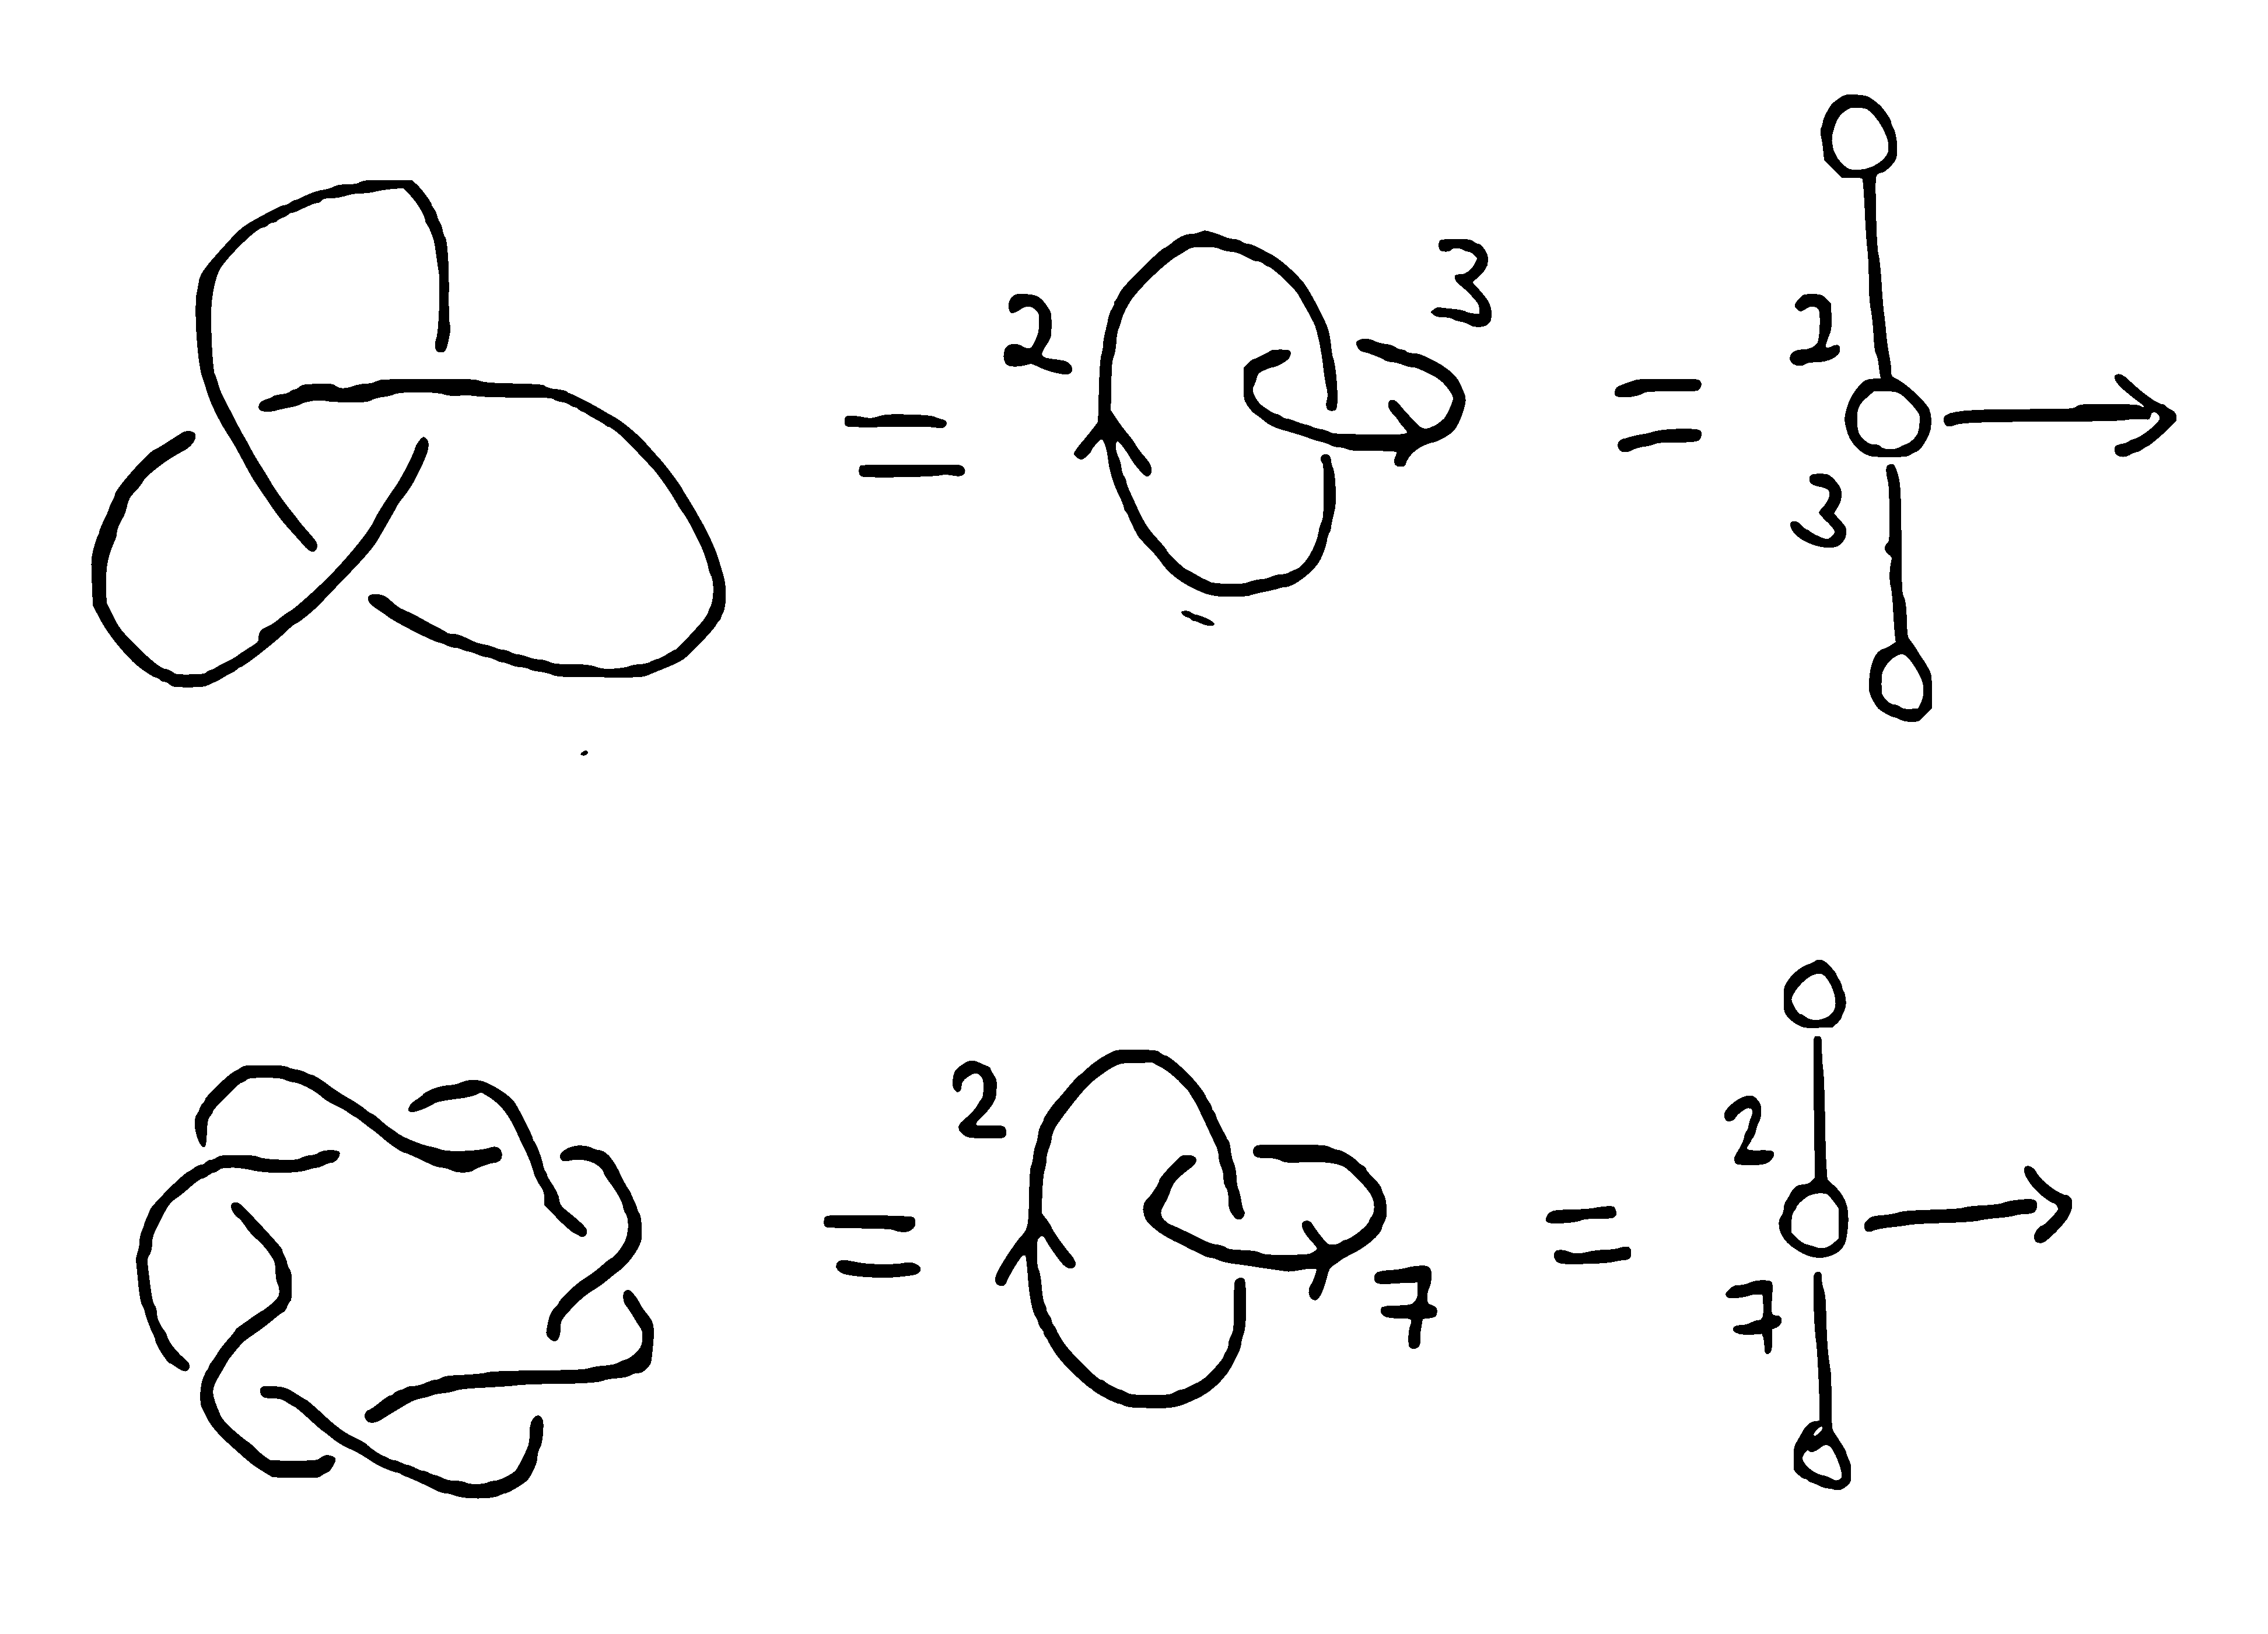
\includegraphics[width=0.5\textwidth]{figures/torussolmuja-homologia-akseleita-ja-pujoskaavioita.pdf}
        \caption{Kaksi torussolmua eri tavoin esitettyinä.}
        \label{kuva:torussolmuja-eri-tavoin}
    \end{figure*}
    Pujoskaaviossa on kolmenlaisia komponentteja, jotka on piirretty alle.
    \begin{center}
        \begin{tikzpicture}
            % --- CRÉATION DES NŒUDS ---
            % Vous positionnez vos nœuds de base ici.
            % On place le symbole \Gamma entre les accolades à la fin
            % \node[rectangle node] (Gamma) at (0,0) {$\Gamma$};
            \node[solid node] (A) at (0,0) {};
            \node[empty node] (B) at (1.5,0) {};
            \node[placeholder] (a) at (1,0) {};
            \node[placeholder] (b) at (2.5,0) {};
            \node[placeholder] (c) at (3,0) {};

            % --- 2 & 5) FLÈCHES VERS LE VIDE ---
            % LaTeX ne peut pas deviner l'espace vide absolu sans direction.
            % La syntaxe "++(angle:distance)" est idéale : vous donnez juste un angle 
            % (ex: 135 degrés) et une longueur (ex: 1cm), et LaTeX calcule 
            % automatiquement la coordonnée finale dans l'espace vide.
            \draw[->, thin] (c) -- ++(0:1cm);

            % --- 3) ARÊTES AVEC VALEURS AUX DEUX EXTRÉMITÉS ---
            % "near start" et "near end" placent les entiers automatiquement aux bouts.
            % L'option "swap" [xxx, yyy, swap] (ou ') permet de basculer le texte de l'autre côté de la ligne.
            \draw (A) -- node[edge value, near start] {$\alpha$}
                        node[edge value, near end] {} (a);
                        
            \draw (B) -- node[edge value, near start] {$\beta$} 
                        node[edge value, near end] {} (b);

        \end{tikzpicture}
    \end{center}
    Tässä $\alpha,\beta$ ovat joitain kokonaislukuja. Merkitään komponentteja tekstin seassa $\bullet,\circ,\rightarrow$. Joissakin tilanteissa on hyödyllistä \emph{juurtaa} kaavio, eli valita mielivaltaisesti jokin silmuista kaavion juureksi. Juurta merkitään $\bullet$. Juurtamaton kaavio sisältää vain tyypillisiä silmuja $\circ$ ja nuolia $\rightarrow$.

    Palloa $\circ$ (tai $\bullet$) käytetään kuvaamaan avaruutta, jossa linkki elää. Jos $\linkki=(\Sigma,\solmu_1)$, niin $\circ$ on $\Sigma$. Tässä työssä $\Sigma$ on aina $\S^3$. Lauseen~\ref{lause:s3-kuidutus} nojalla $\S^3$ voidaan kuiduttaa jollakin epätriviaalilla tavalla. Tämän vuoksi on tarpeellista esittää pallon $\circ$ yhteydessä myös tietoa kuidutuksesta. Jos $k_1,k_2$ ovat kuidutuksen määräävät kokonaisluvut, ts. erityiskuitujen moninkerrat, ilmaistaan tämä pujoskaaviolla
    \begin{center}
        \begin{tikzpicture}
            \node[empty node] (A) at (0,0) {};
            \node[empty node] (k1) at (0,1) {};
            \node[empty node] (k2) at (0,-1) {};

            \draw (A) -- node[edge value, near start] {$k_1$}
                         node[edge value, near end] {} (k1);
            \draw (A) -- node[edge value, near start, swap] {$k_2$}
                         node[edge value, near end] {} (k2);
        \end{tikzpicture}
    \end{center}
    Pallot $\circ$ voikin itse asiassa jakaa kahteen luokkaan: \emph{lehdiksi}, joilla on vain yksi kaari ja \emph{silmuiksi}, joilla voi olla useampi kaari. Silmu symboloi avaruutta $\S^3$ ja lehteä puolestaan avaruuden erityiskuitua. Lehden kaarelle voidaan asettaa kokonaisluku, joka kertoo kyseisen erityiskuidun kertaluvun.

    Teknisesti ottaen triviaalisti kuidutetun avaruuden pujoskaavioon voitaisiin piirtää lehdet siten, että $k_1=k_2=1$, mutta on mielekästä piirtää kaavioista mahdollisimman minimaalisia. Jos $k_2=1$, mutta $k_1>1$, niin avaruudella on vain yksi erituiskuitu, jolloin säännölliset kuidut eivät homologisesti poikkea triviaalista tapauksesta.

    Nuolet $\rightarrow$ vastaavat linkin komponentteja. Nuoli $\rightarrow$ on \emph{aina} kiinnitetty silmuun $\circ$ tai $\bullet$ ja se tarkoittaa jotakin yhtä (mielivaltaista) kuitua avaruudessa, johon se on kiinnitetty. Nuoli voi kuvata säännöllistä kuitua, jolloin sille ei tarvitse antaa kokonaislukua, tai erityiskuitua jolloin sille annetaan kokonaisluku samaan tapaan kuin lehdillekin. On tosin huomattava, että $\S^3$:lla voi olla korkeintaan kaksi erityiskuitua.

    Yksinkertaisin solmu, epäsolmu $\bigcirc\hookrightarrow\S^3$ voidaan esittää kaaviolla
    \begin{center}
        \begin{tikzpicture}
            \node[empty node] (A) at (0,0) {};
            \draw[->, thin] (A) -- ++(0:1cm);
        \end{tikzpicture},
    \end{center}
    jossa $\circ$ vastaa 3-palloa ja $\rightarrow$ siihen upotettua epäsolmua. Jos $\linkki=(\S^3,\solmu_1\cup\cdots\cup\solmu_n)$ ja $\linkki'=(\S^3,\solmu_{n+1}\cup\cdots\cup\solmu_m)$ ovat linkkejä, niin näiden linkkien pujos komponentteja $\solmu_i\in\linkki,\solmu_j\in\linkki'$ myöden voidaan kuvata kaaviolla
    \begin{center}
        \begin{tikzpicture}
            \node[rectangle node] (L1) at (0,0) {$\linkki$};
            \node[text box] (plus) at (1.5,0) {$+$};
            \node[rectangle node] (L2) at (3,0) {$\linkki'$};
            \node[text box] (equals) at (4,0) {$=$};
            \node[rectangle node] (l1) at (5,0) {$\linkki$};
            \node[rectangle node] (l2) at (7,0) {$\linkki'$};

            \draw[->] (L1) -- ++(0:1cm);
            \draw[->] (L2) -- ++(180:1cm);

            \draw (l1) -- node[edge value, near start] {}
                          node[edge value, near end] {} (l2);
        \end{tikzpicture}
    \end{center}
    ja linkeille $\linkki,\linkki'$ voi muodostaa induktiivisesti samoja periaatteita noudattaen omat kaavionsa. Tällaista kaaviota kutsutaan \emph{pujoskaavioksi.}
\end{konstruktio}
\begin{maaritelma}[Pujoskaavio]
    Kutsutaan konstruktiossa~\ref{konstruktio:pujoskaavio} esiteltyjä puuverkkoja \emph{pujoskaavioiksi} ja puuverkkojen erilaisia komponentteja \emph{lehdiksi}, \emph{silmuiksi}, \emph{nuoliksi}, \emph{kaariksi} ja \emph{juuriksi} siten kuin konstruktiossa on kyseisiä sanoja konstruktiossa käytetty.

    Olkoon $\linkki=(\S^3,\solmu_1\cup\cdots\solmu_n)$ linkki. Merkitään linkin pujoskaaviota $\Gamma(\linkki)=\Gamma(m)=\Gamma(m_1,\dots,m_n)$, jossa $m_i$ on solmun $\S_i$ kertaluku. Kertaluvun $m_i$ positiivisuus tai negatiivisuus kertoo solmun suunnistuksen.

    Vastaavasti jos $\Gamma$ on pujoskaavio, olkoon $\linkki(\Gamma)$ kaaviota vastaava linkki.
\end{maaritelma}
\begin{huomautus}
    Annetussa pujoskaavion konstruktiossa ainoa keino välittää informaatiota avaruuksien tai käyrien suunnistuksesta on kuituja kuvaavien kokonaislukujen positiivisuus tai negatiivisuus. Täyden tarkkuuden saavuttamiseksi kaavion pitäisi välittää tietoa myös pohja-avaruuden suunnistuksesta. Lauseessa~\ref{lause:pujoskaaviopläjäys} kuitenkin osoitetaan, että käytännössä avaruuksien voi aina olettaa olevan positiivisesti suunnistettuja.
\end{huomautus}
Kun pujoskaaviot on nyt esitelty, tutkitaan joitakin esimerkkejä.

% Epäsolmujen erillinen solmu
\begin{esimerkki}[Erillinen summa]
    Kahden epäsolmun (tai yleisemmin linkin) erillistä summaa kuvataan erillisillä pujoskaavioilla
    \begin{center}
        \begin{tikzpicture}
            \node[empty node] (A) at (0,0) {};
            \node[empty node] (B) at (1.5,0) {};

            \draw[->] (A) -- ++(0:1cm);
            \draw[->] (B) -- ++(0:1cm);
        \end{tikzpicture}
    \end{center}
\end{esimerkki}
% Kahden epäsolmun pujominen
\begin{esimerkki}
    Esimerkiksi jos kaksi epäsolmua $(\S^3,\solmu_1),(\S^3,\solmu_2)$ pujotaan yhteen, on tuloksena tyhjä $\S^3$ ilman yhtäkään solmua, kuten lemma~\ref{lemma:s3-torushajotus} osoittaa.
    \begin{center}
        \begin{tikzpicture}
            \node[empty node] (A) at (0,0) {};
            \node[text box] (plus) at (1.5,0) {$+$};
            \node[empty node] (B) at (3,0) {};
            \node[text box] (equals1) at (4,0) {$=$};
            \node[empty node] (a) at (5,0) {};
            \node[empty node] (b) at (6.5,0) {};
            \node[text box] (equals2) at (4,-0.75) {$=$};
            \node[empty node] (ab) at (5,-0.75) {};

            \draw[->] (A) -- ++(0:1cm);
            \draw[->] (B) -- ++(180:1cm);
            \draw (a) -- node[edge value, near start] {} 
                         node[edge value, near end] {} (b);
        \end{tikzpicture}
    \end{center}
\end{esimerkki}
Lauseen~\ref{lause:s3-kuidutus} topologisessa todistuksessa tehtiin liimausoperaatio, jossa liimattiin vääntyneitä toruksia. 
\begin{esimerkki}(Torussolmut)
    Torussolmu $\solmu(p,q)\subset\S^3$ voidaan esittää kuidutuksen $\pi_{p,q}:\S^3\to\S^2$ säännöllisenä kuituna. Siispä $(p,q)$-torussolmun pujoskaavio on
    \begin{center}
        \begin{tikzpicture}
            \node[empty node] (A) at (0,0) {};
            \node[empty node] (p) at (0,1) {};
            \node[empty node] (q) at (0,-1) {};

            \draw[->] (A) -- ++(0:1cm);

            \draw (A) -- node[edge value, near start] {$p$}
                         node[edge value, near end] {} (p);
            \draw (A) -- node[edge value, near start, swap] {$q$}
                         node[edge value, near end] {} (q);
        \end{tikzpicture}
    \end{center}
\end{esimerkki}
% S(p,q)=S(q,p) pujoskaavioilla
\begin{esimerkki}
    Lemma~\ref{lemma:pq-torussolmu-on-qp} saa pujoskaavioiden avulla muodon
    \begin{center}
        \begin{tikzpicture}
            \node[empty node] (A) at (0,0) {};
            \node[empty node] (K1) at (0,1) {};
            \node[empty node] (K2) at (0,-1) {};
            \node[text box] (equals) at (2,0) {$=$};
            \node[empty node] (a) at (3.5,0) {};
            \node[empty node] (k1) at (3.5,-1) {};
            \node[empty node] (k2) at (3.5,1) {};

            \draw[->] (A) -- ++(0:1cm);
            \draw[->] (a) -- ++(0:1cm);

            \draw (A) -- node[edge value, near start] {$k_1$}
                         node[edge value, near end] {} (K1);
            \draw (A) -- node[edge value, near start, swap] {$k_2$}
                         node[edge value, near end] {} (K2);
            \draw (a) -- node[edge value, near start, swap] {$k_1$}
                         node[edge value, near end] {} (k1);
            \draw (a) -- node[edge value, near start] {$k_2$}
                         node[edge value, near end] {} (k2);
        \end{tikzpicture}
    \end{center}
\end{esimerkki}
\begin{esimerkki}[Iteroitu torussolmu]
    Kaapeloidaan $(p_1,q_1)$-torussolmu $\solmu$ $(p_2,q_2)$-kaapelilla. Olkoon $\S_1^3$ avaruus, jossa $\solmu$ elää ja $\T\subset\S^3$ torus, jonka pinnalle $\solmu$ voidaan piirtää. Tällöin $\solmu$ kulkee $p_1$ kertaa pituuspiirin ympäri ja $q_1$ kertaa ympäryspiirin ympäri.

    Kaapelin pujoskaavio on
    \begin{center}
        \begin{tikzpicture}
            \node[empty node] (A) at (0,0) {};
            \node[empty node] (p2) at (0,1) {};
            \node[placeholder] (q2) at (-1,0) {};
            \node[placeholder] (k) at (0,-1) {};

            \draw[->] (A) -- ++(180:1cm);
            \draw[->] (A) -- ++(-90:1cm);

            \draw (A) -- node[edge value, near start, swap] {$p_2$}
                         node[edge value, near end] {} (p2);
            \draw (A) -- node[edge value, near start] {$q_2$}
                         node[edge value, near end, swap] {} (q2);
            \draw (A) -- node[edge value, near start] {$1$}
                         node[edge value, near end] {} (k);
        \end{tikzpicture}
    \end{center}
    Kaapeli on kahden solmun linkki. Avaruudella $\S_2^3$, jossa kaapeli elää on, kuidutus $\pi_{p_2,q_2}:\S^3-\S^2$. Solmut avaruudessa ovat säännöllinen kuitu on kertaluvulla 1 (torussolmu $\solmu'=\solmu'(p_2,q_2)$) ja erityiskuitu kertaluvulla $q_2$ (epäsolmu). Jos erityiskuitu eli epäsolmu pujotaan torussolmuun $\solmu(p_1,q_1)$, liimatessa $\S_2^3\setminus\solmu'$ avaruuteen $\S_1^3\setminus\solmu$ täytyy ensimmäistä vääntää niin rajusti, että $\solmu'(p_2,q_2)$ muuttuu iteroiduksi.
    \begin{center}
        \begin{tikzpicture}
            % torussolmu
            \node[empty node] (B) at (0,0) {};
            \node[empty node] (p1) at (0,1) {};
            \node[empty node] (q1) at (0,-1) {};
            \node[placeholder] (arrow1) at (1,0) {};
            % kaapeli
            \node[empty node] (A) at (3,0) {};
            \node[empty node] (p2) at (3,1) {};
            \node[placeholder] (q2) at (2,0) {};
            \node[placeholder] (arrow2) at (3,-1) {};
            % iteroitu torussolmu
            \node[empty node] (b) at (6,0) {};
            \node[empty node] (pp1) at (6,1) {};
            \node[empty node] (qq1) at (6,-1) {};
            \node[empty node] (a) at (8,0) {};
            \node[empty node] (pp2) at (8,1) {};
            \node[placeholder] (arrow3) at (8,-1) {};
            % tekstit
            \node[text box] (plus) at (1.5,0) {$+$};
            \node[text box] (equals) at (4.5,0) {$=$};

            % torussolmu
            \draw[->] (B) -- ++(0:1cm);
            % kaapeli
            \draw[->] (A) -- ++(180:1cm);
            \draw[->] (A) -- ++(-90:1cm);
            % iteroitu torussolmu
            \draw[->] (a) -- ++(-90:1cm);

            % torussolmu
            \draw (B) -- node[edge value, near start] {$p_1$}
                         node[edge value, near end] {} (p1);
            \draw (B) -- node[edge value, near start, swap] {$q_1$}
                         node[edge value, near end] {} (q1);
            \draw (B) -- node[edge value, near start] {$1$}
                         node[edge value, near end] {} (arrow1);
            % kaapeli
            \draw (A) -- node[edge value, near start, swap] {$p_2$}
                         node[edge value, near end] {} (p2);
            \draw (A) -- node[edge value, near start, swap] {$q_2$}
                         node[edge value, near end] {} (q2);
            \draw (A) -- node[edge value, near start] {$1$}
                         node[edge value, near end] {} (arrow2);
            % iteroitu torussolmu
            \draw (b) -- node[edge value, near start] {$p_1$}
                         node[edge value, near end] {} (pp1);
            \draw (b) -- node[edge value, near start, swap] {$q_1$}
                         node[edge value, near end] {} (qq1);
            \draw (b) -- node[edge value, near start] {$1$}
                         node[edge value, near end] {$q_2$} (a);
            \draw (a) -- node[edge value, near start, swap] {$p_2$}
                         node[edge value, near end] {} (pp2);
            \draw (a) -- node[edge value, near start] {$1$}
                         node[edge value, near end] {} (arrow3);
        \end{tikzpicture}
    \end{center}
\end{esimerkki}

\subsection{Pujoskaavioiden ominaisuuksia}
Tässä kappaleessa käsitellään muodollisesti pujoskaavioiden ominaisuuksia ja todistetaan joitakin hyödyllisiä tuloksia.
\begin{propositio}
    Linkki $\linkki=(\Sigma,K)$ on kompleksitason käyrän singulariteetin linkki jos ja vain jos sillä on yhtenäinen pujoskaavio, jonka kaikki painot ja kaarideterminantit ovat positiivisia. Tällöin sillä on minimaalinen pujoskaavio näillä ominaisuuksilla.
\end{propositio}
\begin{proof}
    En tiedä.
\end{proof}
\begin{lemma}
    Kahden linkin osasen (virtuaalisen tai todellisen) linkkiluku $\Sigma$:ssa saadaan laskemalla pujoskaaviossa osasten välillä olevan polun viereisten painojen tulo.
\end{lemma}
\begin{proof}
    En tiedä.
\end{proof}

\begin{propositio}
    Polynomisolmun pujoskaavion sidoskertoimet saadaan kaavoista $\alpha_1=q_1$ ja $\alpha_{i+1}=q_{i+1}+q_i p_i p_{i+1}$, missä $p_i,q_i$ ovat polynomin Puiseux-dataa.
\end{propositio}
\begin{proof}
    \citep{EN1985}[Prop 1A.1]
\end{proof}


\subsection{Monimutkainen esimerkki}
Tässä kappaleessa tutustutaan monimutkaiseen solmuun ja sen pujoskaavion rakentamiseen sekä mielellään myös toisin päin.

\section{Dehnin kirurgia}
Työssä on tähän asti nojattu runsaasti yksinkertaisiin 3-monistoihin, pääosin $\S^3$:een. Monimutkaisempia 3-monistoja ja edistyneempää monistojen teoriaa on pyritty tarkoituksella häivyttämään, jotta vastaavasti fokus työn kannalta keskeisiin rakenteisiin pysyisi kirkkaana.

Itse asiassa solmut ja pujominen löytyvät modernissa matemaattisessa kirjallisuudessa paljon laajemmasta 3-monistojen hajotelmien kontekstista. 
\section{RPI-kaaviot äärettömyydessä}
Tässä osiossa rakennetaan edellisten avulla ensin RPI-kaaviot ja sitten päätulos.

\subsection{Algebrallisen käyrän pujoskaavio}
Määritellään ensin juurretut kaaviot. Usein hyödyttää käsitellä juurrettuja pujoskaavioita, joilla on jokin juurisilmu. Tässä työssä käsitellyn teorian kontekstissa ei ole matemaattisesti oikeaa tapaa määrittää, minkä silmuista pitäisi olla kaavion juuri. Juuren valinta on siis epämatemaattinen ja perustuu johonkin intuitivistiseen syyhyn (joka yleensä on kontekstista selvä). Juurretun kaavion etu on se, että juuri antaa kaaviolle ``relativistisen koordinaatiston''.
\begin{maaritelma}
    Olkoon $\Omega$ pujoskaavio. $\Omega$ on \emph{juurrettu}, jos jokin sen silmuista, joka ei ole lehti, valitaan kaavion juureksi.
\end{maaritelma}
Millä tavalla juurretty kaavio sitten antaa relativistisen koordinaatiston? Määritellään jokaiselle pujoskaavion kaarelle lähi- ja kaukopää.
\begin{maaritelma}
    Olkoon $\Omega$ juurrettu pujoskaavio. Olkoon $v$ jokin kaari ja $l,k$ kaaren silmut. Kuljettakoon kummastakin silmusta lyhyin reitti (matkalla olevien silmujen määrässä mitattuna) kaavion juuren luo, ja olkoon $\gamma(\cdot)\in\N$ matkalla olevien silmujen määrä alkupiste $l$ tai $k$ poislukien. Jos
    \begin{equation*}
        \gamma(l)<\gamma(k),
    \end{equation*}
    niin $l$ on $v$:n \emph{lähipää} ja $k$ sen \emph{kaukopää}. Päitä vastaavia painoja kutsutaan samaten \emph{lähi-} ja \emph{kaukopainoiksi}.
\end{maaritelma}
\begin{huomautus}
    Lukijan on syytä huomata, että $\gamma(l)\ne\gamma(k)$ aina, sillä muutoin kaaviossa olisi silmukka.
\end{huomautus}
Rajoittamalla tutkimus sopivan hyvin käyttäytyviin kaavioihin löytyy yksinkertainen vastaavuus algebrallisten painojen ja pujoskaavioiden välillä. Tällainen kaavio on RPI-pujoskaavio.
\begin{maaritelma}
    Olkoon $\Omega$ juurrettu pujoskaavio. $\Omega$ on \emph{RPI-pujoskaavio} (englannista \emph{Reverse Puiseux Inequalities}, käänteiset Puiseux-epäyhtälöt), jos
    \begin{enumerate}
        \item jokaisella silmulla on korkeintaan yksi lähipaino, joka ei ole 1,
        \item kaikki lähipainot ovat positiivisia ja
        \item kaikki kaarideterminantit ovat negatiivisia, mukaanlukien juurisilmun kaaret tapauksessa $n=1$ ja muutoin.
    \end{enumerate}
\end{maaritelma}

Algebrallisten käyrien kannalta kiinnostavaa on ymmärtää, miten käyrä käyttäytyy äärettömyydessä. On mahdollista määritellä mielekkäällä tavalla käyrän linkki äärettömyydessä, käyttäen samoja ideoita kuin määritellessä käyrän linkkiä sen singulariteetissa.

\par\vspace{\topsep}
\noindent
\textbf{Lause \ref{lause:päätulos}.} \emph{(i) Pelkistetty algebrallinen käyrä $V\subset\C^2$ jollakin upotuksella $\C^2\subset\P^2$ määrittää RPI-pujoskaavion $\Omega$ $V$:n äärettömyyslinkille. Äärettömyyspisteiden lukumäärälle pätee $n_\infty(V)=n$, missä $n$ on kaavion juurisilmun valenssi. Lisäksi $\deg(V)=\ell_\text{root}$, jossa $\ell_\text{root}$ on juuren (virtuaalisen) komponentin linkkiluku äärettömyyslinkin kanssa. Jos $V$ on säännöllinen käyrä, $\Omega$ on säännöllinen (määritelmä???) pujoskaavio.}

\emph{(ii) Linkki on jonkin äärettömyyslinkin (joka voidaan valita säännölliseksi (määritelmä???), jopa hyväksi (määritelmä???)) osalinkki jos ja vain jos sillä on RPI-pujoskaavio.}
\begin{ajatus}
    Lause on sangen tiukasti muotoiltu, mutta sen ydinajatus on seuraava.
    \begin{enumerate}[i]
        \item Minkälainen solmu tai pujoskaavio algebrallisella käyrällä on?
        \item Millä ehdoilla algebralliset käyrät vastaavat linkkejä ja pujoskaavioita yksi yhteen?
    \end{enumerate}
\end{ajatus}
\begin{proof}[Lausen \ref{lause:päätulos}(i) todistus]
    Tarkastelun kohteena ovat käyrät $V$, joilla on upotus $V\hookrightarrow\C^2$, missä kompleksiavaruudella on jokin sopiva upotus projektiiviseen tasoon $\C^2\hookrightarrow\P^2$. $V$:llä on olemassa jokin projektiivinen laajennus $C$, joka myös saattaa saada erisuuria arvoja äärettömyydessä riippuen $V$:n haarojen asymptotiikasta.

    Tarkemmin sanottuna $V=C-(C\cap\P^1)\subset\P^2-\P^1=\C^2$, missä $C$ on jokin pelkistetty\footnote{Ei toistuvia pelkistymättömiä komponentteja} projektiivinen käyrä. Jos oletetaan, että $\P^1$ ei ole käyrän $C$ komponentti, niin
    \begin{equation*}
        C\cap\P^1=\{P_1,\dots,P_n\},\quad n<\infty,
    \end{equation*}
    sillä myös $\P^1$ voidaan nähdä algebrallisena käyränä $\P^2$:ssa. Olkoon $D'\hookrightarrow\P^1$ siten, että $C\cap\P^1\subset D'$ leikkauspisteet sisältävä levy. Olkoon $D$ $\P^2$:ssa säännöllinen (määritelmä???) 4-levy-ympäristö $D'$:lle, siten että reuna $R=\partial D$ leikkaa $C$:n ja $\P^1$:n transversaalisesti (määritelmä???).

    Tällöin $\linkki_0=(R,(\P^1\cup C)\cap R)$ on linkki, jota voidaan esittää pujoskaaviolla
    \begin{equation*}
        \Gamma=K_0\xleftarrow{0}
        \begin{cases}
            1,\quad\Gamma_1 \\
            \dots \\
            1,\quad\Gamma_n
        \end{cases}
    \end{equation*}
    selitystä\dots

    
\end{proof}


\input{sections/n-yhteenveto.tex}


%% LÄHDELUETTELO
%%  BibTeX-tiedoston kokoaminen onnistuu näppärästi esim. 
%%  Firefoxin/Chromen Zotero-lisäosalla http://www.zotero.org/
%%  joka osaa poimia viitteet suoraan Google Scholarista.

%% Ladataan library.bib
\bibliography{library}

%% Liitteet
%% Poista a.o. \clearpage-, \thesisappendix- ja input -makrot, jos liiteitä ei ole.
\clearpage
\thesisappendix

\section{Esimerkki liitteestä\label{LiiteA}}

Liitteet eivät ole opinnäytteen kannalta välttämättömiä ja 
opinnäytteen tekijän on 
kirjoittamaan ryhtyessään hyvä ajatella pärjäävänsä ilman liitteitä.
Kokemattomat kirjoittajat, jotka ovat huolissaan
tekstiosan pituudesta, paisuttavat turhan 
helposti liitteitä pitääkseen tekstiosan pituuden annetuissa rajoissa.
Tällä tavalla ei synny hyvää opinnäytettä.   

Liite on itsenäinen kokonaisuus, vaikka se täydentääkin tekstiosaa.
Liite ei siten ole pelkkä listaus, kuva tai taulukko, vaan 
liitteessä selitetään aina sisällön laatu ja tarkoitus. 

Liitteeseen voi laittaa esimerkiksi listauksia. Alla on 
listausesimerkki tämän liitteen luomisesta. 

%% Verbatim-ympäristö ei muotoile tai tavuta tekstiä. Fontti on monospace.
%% Verbatim-ympäristön sisällä annettuja komentoja ei LaTeX käsittele. 
%% Vasta \end{verbatim}-komennon jälkeen jatketaan käsittelyä.
\begin{verbatim}
	\clearpage
	\appendix
	\addcontentsline{toc}{section}{Liite A}
	\section*{Liite A}
	...
	\thispagestyle{empty}
	...
	tekstiä
	...
	\clearpage
\end{verbatim}

Kaavojen numerointi muodostaa liitteissä oman kokonaisuutensa:
\begin{align}
d \wedge A &= F, \label{liitekaava1}\\
d \wedge F &= 0. \label{liitekaava2}
\end{align}


\clearpage
\section{Toinen esimerkki liitteestä\label{LiiteB}}

%% Liitteiden kaavat, taulukot ja kuvat numeroidaan omana kokonaisuutenaan

Liitteissä voi myös olla kuvia, jotka
eivät sovi leipätekstin joukkoon:
%% Ympäristön figure parametrit htb pakottavat
%% kuvan tähän, eikä LaTeX yritä siirrellä niitä
%% hyväksi katsomaansa paikkaan. 
%% Ympäristöä center voi käyttää \centering-
%% komennon sijaan
%%
%\begin{figure*}[htb]
%\centering
%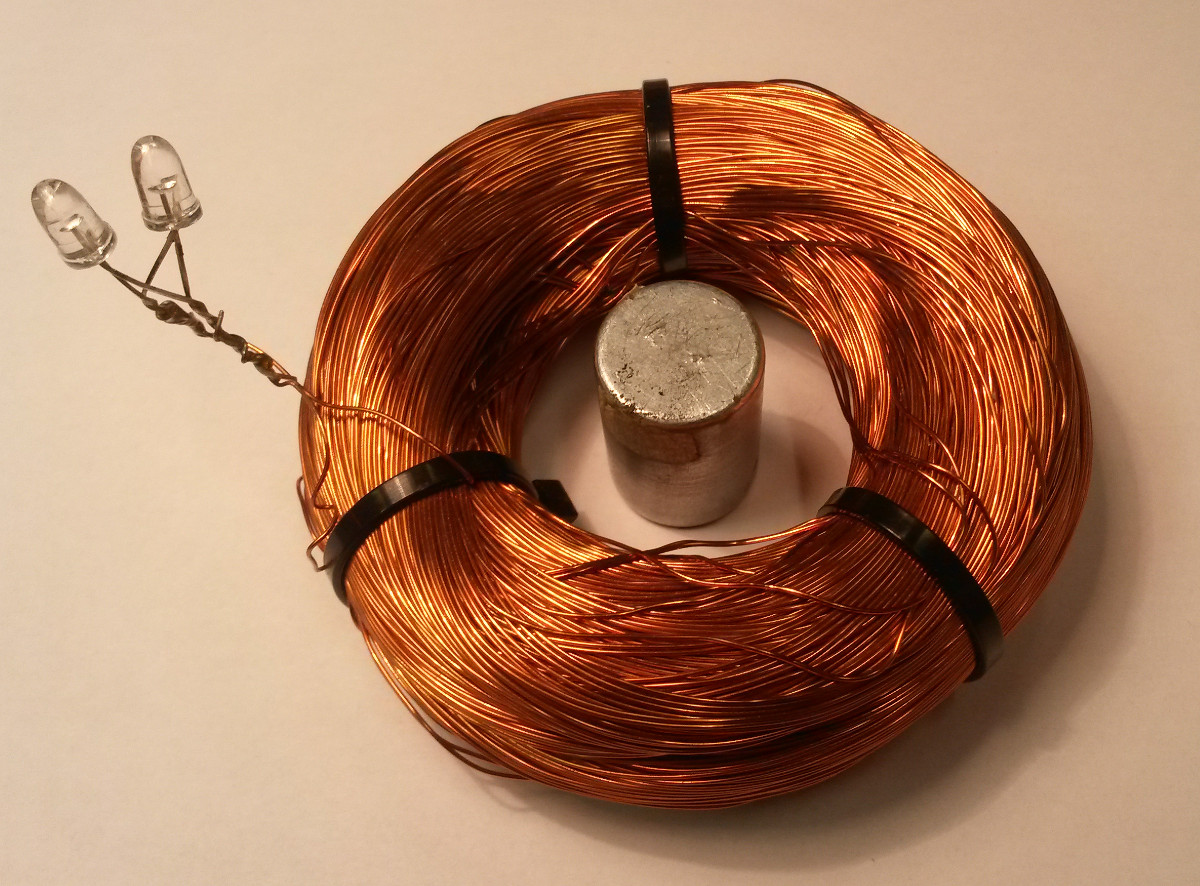
\includegraphics[height=8cm]{figures/ledspole.jpg}
%\caption{Kuvateksti, jossa on liitteen numerointi}
%\label{liitekuva}
%\end{figure*}
%%
Liitteiden taulukoiden numerointi on kuvien ja kaavojen kaltainen:
\begin{table}[htb]
\caption{Taulukon kuvateksti.}
\label{liitetaulukko}
\centering
\begin{tabular}{|lp{0.5\linewidth}|}
\hline
9.00--9.55  & Käytettävyystestauksen tiedotustilaisuus (osanottajat
ovat saaneet sähköpostitse valmistautumistehtävät, joten tiedotustilaisuus
voidaan pitää lyhyenä).\\
9.55--10.00 & Testausalueelle siirtyminen \\
\hline
\end{tabular}
\end{table}
Kaavojen numerointi muodostaa liitteissä oman kokonaisuutensa:
\begin{align}
T_{ik} &= -p g_{ik} + w u_i u_k + \tau_{ik},  \label{liitekaava3} \\
n_i    &= n u_i + v_i.                      \label{liitekaava4}
\end{align}

\clearpage
\section{Matemaattisten lauseiden todistukset\label{LiiteC}}
Systeemianalyysin töissä matemaattisten lauseiden todistukset laitetaan yleensä liitteiksi. Leipätekstissä lauseen yhteydessä todistuksen todetaan löytyyvän liitteestä XX. Tämä ei koske matematiikan töitä, joissa lauseiden todistukset voivat olla merkittävä osa varsinaista työtä!
\begin{maaritelma}
Tässä määritellään $1=1$.
\end{maaritelma}

\begin{lause}[Roposen lause]\label{thrm:roponen}
Lukiomatematiikassa kolmannen asteen yhtälöillä on aina vähintään yksi kokonaislukuratkaisu välillä $[-3,3]$.
\end{lause}
\begin{proof}
Jätetään harjoitustehtäväksi.
\end{proof}

\begin{huomautus}
Lause \ref{thrm:roponen} saattaa olla väärin.
\end{huomautus}

Tiedoston opinnaytepohja.tex alusta löytyy myös muita teoreema- ym. tyylejä sekä suomeksi että englanniksi, joten katso löytyykö sieltä käyttöösi sopiva. Voit myös määritellä itse lisää.

\end{document}
